\documentclass[12pt, a4paper]{article}
\usepackage[utf8]{inputenc}
\usepackage{graphicx}
\usepackage{blindtext}
\usepackage{subcaption}
\usepackage{wrapfig}
\usepackage{adjustbox}
%\usepackage[square,numbers]{natbib}
\usepackage{url}
\usepackage{listings}
\usepackage{amsmath}
\usepackage{amsfonts}
\usepackage{placeins}

\renewcommand{\tablename}{Tablo}
\renewcommand{\figurename}{Şekil}
\renewcommand{\refname}{Kaynakça}
\renewcommand{\contentsname}{İçindekiler}
\title{\textbf{GAN Metodu ile Yüz Oluşturma}}
\author{Elif Filiz}
\date{07.03.2024}
\begin{document}
	\thispagestyle{empty}
	\maketitle 
	
	\textbf{KÜTAHYA SAĞLIK BİLİMLERİ ÜNİVERSİTESİ}\centering
	\begin{figure}[!h]
		\centering
		
\includegraphics{ksbu}
	\end{figure}
	\newpage
	\tableofcontents
	\newpage
	
	\raggedright
	\section{Özet}

	Bu çalışmanın amacı, CelebA veri seti kullanılarak farklı GAN türleri ile rastgele insan yüzleri üretmek ve bu süreçte türlerin kullanımındaki asıl amacın ne olduğu ve mimarilerini anlamaktır..
	
	\section{Giriş}
	
	Bu çalışma, Generative Adversarial Networks (GAN) yöntemlerini kullanarak CelebA veri setiyle rastgele insan yüzleri oluşturma üzerine odaklanmaktadır. GAN'ler, veri setlerindeki örüntüleri öğrenerek yeni ve özgün veri örnekleri oluşturabilen güçlü yapay zeka modelleridir. Bu projede, farklı GAN türleri kullanılarak gerçekçi ve yüksek kaliteli insan yüzleri üretilmiş ve bu yöntemlerin performansları karşılaştırılmıştır.
	
	CelebA veri seti kullanılarak çeşitli GAN modelleri (örneğin DCGAN, CGAN, CycleGAN ve StyleGAN) başarıyla eğitilmiş ve her bir modelin yüz üretimindeki başarımı değerlendirilmiştir. Ayrıca her modelin yapıları incelenmiş ve aralarındaki farklar öğrenilmiştir.
	
	Farklı GAN türlerinin performansları karşılaştırılmış ve hangi modelin en iyi sonuçları verdiği belirlenmiştir. Bu karşılaştırma, ileride yapılacak benzer çalışmalara rehberlik edebilecek önemli bulgular sunmaktadır.
	
	Özellikle insan yüzlerinin özelliklerini daha detaylı ve gerçekçi bir şekilde yakalayabilen yenilikçi GAN yapıları üzerine odaklanılmış ve bu yapıların sunduğu avantajlar değerlendirilmiştir.
	
	Çalışmanın temel amacı, farklı GAN türlerini kullanarak yüksek kaliteli ve gerçekçi insan yüzleri oluşturmak ve bu modellerin performanslarını karşılaştırmaktır. StyleGAN ve StyleGAN2 gibi gelişmiş GAN modellerinin etkinliğini değerlendirerek, en iyi performans gösteren modeli belirlemek ve uygulama alanlarına yönelik önerilerde bulunmak bu çalışmanın odak noktalarını oluşturmuştur.
	
	Çalışma motivasyonu günümüz yapay zeka teknolojilerinin potansiyelini keşfetmek ve özellikle Generative Adversarial Networks (GAN) kullanarak yüksek kaliteli ve gerçekçi insan yüzleri oluşturmanın yollarını araştırmaktır. GAN'lerin ürettiği görsellerin kalitesi ve gerçekçiliği, bu modellerin medya, eğlence, güvenlik ve sağlık gibi çeşitli alanlarda geniş uygulama potansiyeline sahip olduğunu göstermektedir. Bu nedenle, bu teknoloji üzerine çalışmak, hem akademik bilgi birikimimizi artırmak hem de endüstriyel uygulamalara katkı sağlamak açısından önemlidir.
	
	Bu çalışmada ele aldığım problem, mevcut GAN modellerinin insan yüzü üretiminde yaşadığı zorlukları ve bu zorlukları aşarak daha gerçekçi ve kaliteli yüzler üretme yollarını araştırmaktır. 
	
	Özellikle çözmeye ve geliştirmeye çalıştığım yönler şunlardır: Mevcut GAN modelleri ile üretilen yüzlerin bazen bulanık, yapay ya da gerçekçilikten uzak olması gibi problemleri çözerek, daha yüksek kaliteli ve gerçekçi yüzler üretmek, farklı GAN türlerinin performanslarını karşılaştırarak, hangi modellerin hangi koşullarda en iyi sonuçları verdiğini belirlemek ve bu modellerin eğitim süreçlerini optimize etmek, üretilen yüzlerin çeşitliliğini ve özgünlüğünü artırmak, böylece farklı yüz özelliklerini kapsayan daha geniş bir yüz veri tabanı oluşturmak, GAN modellerinin eğitim süreçlerindeki hesaplama maliyetlerini ve zamanını azaltarak, daha verimli ve hızlı bir model geliştirme süreci sağlamak.
	
	\section{Literatür Araştırması}
	
	CelebA veri seti kullanılarak farklı GAN modelleri (DCGAN, WGAN, StyleGAN) başarıyla eğitildi ve her bir modelin performansı karşılaştırıldı.
	
	GAN modellerinin eğitim süreçleri optimize edildi ve daha hızlı ve verimli eğitim süreçleri geliştirildi. Bu, hesaplama maliyetlerini ve eğitim sürelerini azaltmamıza yardımcı oldu.
	
	Farklı GAN modellerinin güçlü ve zayıf yönlerini belirleyerek, hangi modellerin hangi koşullarda en iyi sonuçları verdiği ortaya koyuldu. Bu karşılaştırmalı çalışma, gelecekteki araştırmalara ve uygulamalara rehberlik edebilecek önemli bulgular sundu.
	
	\subsection{Üretken Çekişmeli Ağın(GAN) Matematiksel Denklemi}
	
	\begin{equation}
		\begin{aligned}
			& \min_{G} \max_{D} V(D,G) = 
			& \mathbb{E}_{x\sim\mu}[\log(D(x))] + \mathbb{E}_{z\sim\gamma}[\log(1 - D(G(z)))]
		\end{aligned}
		\label{Gan'ın matematiksel formülü}
	\end{equation}
	
	Formül \eqref{Gan'ın matematiksel formülü}'de Gan'ın Matematiksel Denklemi verilmiştir\cite{yilmaz2023understanding}.
	
	$\gamma$ = Gürültünün veri dağılımı
	
	$\mu$ = Veri kümesindeki gibi orijinal veri dağılımı
	
	${x\sim\mu}$ = $\mu$'dan örneklenen veriler
	
	${z\sim\gamma}$ = $\gamma$'dan örneklenen veriler
	
	D(x) = Görüntünün gerçek olma olasılığı
	
	z = Rastgele gürültü örneği
	
	G(z) = Bir gürültü örneği kullanılarak oluşturulan görüntü
	
	D(x)'in görüntünün gerçek olma olasılığını gösterdiğini biliyoruz , dolayısıyla Ayırıcı(discriminator) her zaman D(x)'i maksimuma çıkarmak ister , dolayısıyla log(D(x)) maksimuma çıkarılmalı ve İlk bölüm maksimuma çıkarılmalıdır.
	
	Oluşturucu(generator) her zaman ayırıcının oluşturulan görüntülere aldanma olasılığını en üst düzeye çıkarmak ister. Bu, oluşturucunun D(G(z))'yi maksimuma çıkarmak istemesi gerektiği anlamına gelir, dolayısıyla 1- D(G(z))'yi ve dolayısıyla log(1- D(G(z)))'yi minimuma indirmelidir\cite{Celebrity-2024-04-16}.
	
	\subsection{GAN Nedir?}
	
	iki sinir ağının tahminlerinde daha doğru olmak için derin öğrenme yöntemlerini kullanarak birbirleriyle rekabet ettiği bir makine öğrenimi (ML) modelidir\cite{What-2024-05-31}. 
	
	Bir GAN'ı oluşturan iki sinir ağı jeneratör ve diskriminatör olarak adlandırılır. Üreteç evrişimli bir sinir ağı, ayrıştırıcı ise evrişimsiz bir sinir ağıdır. Üretecin amacı, gerçek verilerle kolayca karıştırılabilecek yapay çıktılar üretmektir. Ayırıcının amacı ise aldığı çıktılardan hangilerinin yapay olarak oluşturulduğunu tespit etmektir.
	
	Bir eğitim seti verildiğinde bu teknik, eğitim seti ile aynı istatistiklere sahip yeni veriler üretmeyi öğrenir. Örneğin, fotoğraflar konusunda eğitilmiş bir GAN, insan gözlemcilere en azından yüzeysel olarak özgün görünen ve pek çok gerçekçi özelliğe sahip yeni fotoğraflar üretebilir\cite{Generative-2024-05-31}. 
	
	\subsection{GAN Modelini Eğitme}
	Eğitim sırasında GAN iki girdi alır; rastgele gürültü verileri ve etiketlenmemiş bir giriş verisi. Bu iki girişi kullanarak giriş verilerine benzeyen veriler üretir. GAN'a gelen tüm girişler etiketlenmediğinden GAN, bir tür denetimsiz makine öğrenimidir.
	
	Ayırıcı eğitim aşamasında oluşturucuyu sabit tutuyoruz. Ayırıcı eğitim, gerçek verilerin sahteden nasıl ayırt edileceğini anlamaya çalışırken, oluşturucunun(generator) kusurlarını nasıl tanımlayacağını öğrenmelidir. Bu, kapsamlı şekilde eğitilmiş bir oluşturucuda rastgele çıkış üreten eğitimsiz bir oluşturucudan farklı bir sorundur.
	
	Benzer şekilde, oluşturucu eğitim aşaması sırasında ayırıcıyı sabit tutuyoruz. Aksi halde, oluşturucu hareket etmeye çalışan bir hedefe ulaşmaya çalışır ve asla ilerlemeyebilir.
	
	Gerçek veriler gösterilir ve 1'e yakın çıkış değerleri verecek şekilde eğitilmelidir. Sahte veriler (oluşturucu tarafından oluşturulan) gösterilir ve 0'a yakın çıkış değerleri verecek şekilde eğitilmelidir.
	
	Eğitim sırasında oluşturucu, ayırıcının gerçek verilerden ayırt edemeyeceği veriler üreterek ayırıcıyı kandırmaya çalışır.
	Oluşturucu, ayırıcıdan gelen geri bildirime göre ağırlıklarını günceller. Ayırıcı, oluşturulan veriyi sahte olarak doğru bir şekilde tanımlarsa, oluşturucu bir sonraki yineleme sırasında daha ikna edici veriler üretmek için ağırlıklarını ayarlar.
	Süreç, oluşturucunun sürekli olarak gelişmeye çalıştığı, sonunda gerçek verilerden neredeyse ayırt edilemeyecek veriler üretmeyi hedeflediği bir tür “oyundur”\cite{Multiverse}.
	
	\subsection{NVIDIA StyleGAN nedir?}
	NVIDIA StyleGAN, yüksek kaliteli ve yaratıcı görüntü sentezlemesi için kullanılan bir yapay zeka modelidir. StyleGAN, "Generative Adversarial Networks" (GANs) olarak bilinen bir tür derin öğrenme modeli üzerine kurulmuştur.
	
	GAN'lar, rastgele veriler üretmek için bir oluşturucu model ve bu verileri değerlendirmek için bir ayırıcı model arasında rekabetçi bir ilişki kurar. StyleGAN ise GAN'ların bu mimarisini geliştirir ve daha kaliteli, gerçekçi ve kontrol edilebilir görüntü sentezi sağlar.
	
	StyleGAN'ın özgün özelliği, görüntüyü üretirken stil ve yapı arasında ayrım yapabilmesidir. Bu sayede, oluşturulan görüntülerin farklı yüzler, nesneler veya manzaralar gibi belirli özellikleri kontrol edilebilir. Örneğin, StyleGAN, belirli bir yüzü modifiye edebilir veya farklı saç stilleri, göz renkleri, cilt tonları vb. ekleyebilir.
	
	NVIDIA StyleGAN, özellikle sanat, moda ve diğer yaratıcı alanlarda kullanılan birçok uygulama için popülerdir. Yüksek çözünürlüklü ve gerçekçi görüntüler üretebilir, yeni sanat eserleri oluşturmak veya belirli bir tarzda görüntü sentezi yapmak için kullanılabilir.
	\begin{figure}[h]
		\centering
		\includegraphics[width=0.7\textwidth]{stylegan3}
		\label{stylegan3}
		\caption{Alias-Free Generative Adversarial Networks (StyleGAN3)\cite{-2024-05-31}}
	\end{figure}
	\FloatBarrier
	\subsection{StyleGAN2 ve StyleGAN3 Arasındaki Fark}
	StyleGAN2 ve StyleGAN3'de hizalanmamış FFHQ-U veri kümesi üzerinde eğitilmiş oluşturucular kullanılarak oluşturulan iki "sinemagrafta" "doku yapışması(“texture sticking”)" sorunu için StyleGAN3'ün daha tutarlı bir görüntü oluşturduğu tespit edilmiştir. Yüz onun altında hareket ederken StyleGAN2 sonucunun (solda) ayrıntılarının (saçlar, kırışıklıklar vb.) ekran koordinatlarına nasıl yapıştırılmış gibi göründüğünü, bu sırada tüm ayrıntıların sonucumuzda (sağda) tutarlı bir şekilde dönüştüğü gözlemlenir.
	
	Flickr-Faces-HQ (FFHQ)\cite{karras2019style}, 1024×1024 çözünürlükte 70.000 yüksek kaliteli PNG görüntüsünden oluşur ve yaş, etnik köken ve görüntü arka planı açısından önemli farklılıklar içerir. Ayrıca gözlük, güneş gözlüğü, şapka vb. gibi aksesuarların kapsamı da geniştir. Görüntüler Flickr'dan taranmıştır, dolayısıyla o web sitesinin tüm önyargıları miras alınmıştır ve dlib kullanılarak otomatik olarak hizalanıp kırpılmıştır. Yalnızca izin verilen lisanslar kapsamındaki görseller toplandı. Seti sadeleştirmek için çeşitli otomatik filtreler kullanıldı ve son olarak ara sıra ortaya çıkan heykelleri, tabloları veya fotoğraf fotoğraflarını kaldırmak için Amazon Mechanical Turk kullanıldı.
	
	Amazon Mechanical Turk, Amazon'un 3 Kasım 2005 itibarıyla kullanıcılarına sunmuş olduğu soru-cevap hizmetidir. 
	\begin{enumerate}
		\item \textbf{Model Mimarisi ve Performans}: StyleGAN3, StyleGAN2'nin mimarisini temel alır ancak bazı önemli iyileştirmeler getirir. Özellikle, StyleGAN3, daha iyi eğitim kararlılığı ve daha hızlı eğitim süreçleri sağlayan yeni bir eğitim algoritması olan Adaptive Training gibi özelliklerle gelir. Bu, daha kaliteli ve daha hızlı görüntü sentezi sağlar.
		
		\item \textbf{Daha Yüksek Kalite ve Çözünürlük}: StyleGAN3, daha yüksek kaliteli ve daha yüksek çözünürlüklü görüntüler üretme yeteneğine sahiptir. Önceki model olan StyleGAN2 bile oldukça başarılı olsa da, StyleGAN3, daha gerçekçi ve daha ayrıntılı sonuçlar sağlar.
		
		\item \textbf{Hassas Kontrol ve Düzgün İleri Yayılma (Smooth Forward Spread)}: StyleGAN3, kullanıcılara daha fazla kontrole ve özgürlüğe izin veren daha iyi bir düzgün ileri yayılma özelliğine sahiptir. Bu, belirli özellikleri (örneğin, yüz ifadeleri, nesne özellikleri) daha hassas bir şekilde kontrol etmeyi sağlar ve istenmeyen sonuçların daha az olmasını sağlar.
		
		\item \textbf{Verimlilik ve Hafıza Kullanımı}: StyleGAN3, daha etkili bellek kullanımı ve daha verimli bir algoritma ile gelir. Bu, daha büyük veri kümeleri üzerinde çalışırken daha az bellek tüketimine ve daha hızlı eğitim sürelerine yol açar.
		
		\item \textbf{Topluluk Katılımı ve Geliştirme}: NVIDIA, StyleGAN3'ü geliştirme sürecine daha fazla topluluk katılımı ve geri bildirim alarak şekillendirme eğilimindedir. Bu, modelin daha geniş bir kullanıcı tabanının ihtiyaçlarını ve geri bildirimlerini dikkate alarak gelişmesini sağlar.
		
	\end{enumerate}
	
	\begin{figure}[h]
		\centering
		\includegraphics[width=1\textwidth]{EQ-T}		
		\caption{Çeviri eşdeğerliğinin görselleştirilmesi (EQ-T)\cite{-2024-05-31}}
		\label{EQ-T}
	\end{figure}
	
	Şekil \ref{EQ-T}'de, çeşitli "köprü" konfigürasyonlarında öteleme eşdeğerliğini veya bunun eksikliğini göstermektedir ve EQ-T eşdeğerlik puanlarının anlamını görsel olarak göstermeyi amaçlamaktadır. EQ-T eşdeğerlik puanının arttıkça görsellerdeki gürültünün gittiği ve görüntünün mükemmelleştiği söylenebilir. Görüldüğü gibi 60 dB aralığındaki EQ-T skorları görsel olarak mükemmel\cite{-2024-05-31}.
	
	\clearpage
	\begin{figure}[h]
		\centering
		\includegraphics[width=0.5\textwidth]{dönme}
		\caption{Döndürme denkliğinin görselleştirilmesi (EQ-R)\cite{-2024-05-31}}
		\label{EQ-R}
	\end{figure}
	
	Şekil \ref{EQ-R}'de, Şekil \ref{EQ-T}'e benzer şekilde dönüş eşitliğini göstermektedir. Yalnızca çeviri eşitliği için tasarlanan StyleGAN3-T'miz beklendiği gibi tamamen başarısız oluyor. Aşağıdaki karşılaştırma yöntemi, dönme eşitliği için p4 simetrik G-CNN kullanan StyleGAN3-T'nin bir çeşididir. Model, dönüşün 90 derecenin katlarında kesin olduğu ancak ara açılarda bozulduğu döngüsel bir davranış göstermektedir. StyleGAN3-R ürünümüz, görsel olarak mükemmel olmasa da, yüksek kalitede rotasyon eşitliğine sahiptir.
	
	\subsection{DCGAN Nedir?}
	
	DCGAN, derin evrişimli üretken çekişmeli ağ(Deep Convolutional GAN) anlamına gelir. Bir oluşturucu ve bir ayırıcı kullanılır.
	
	\begin{figure}[h]
		\centering
		\includegraphics[width=0.6\textwidth]{dcganmimari}
		\label{dcganmimari}
		\caption{DCGAN Üretici Katmanları\cite{Train-2024-05-06}}
	\end{figure}
	\FloatBarrier
	DCGAN'lar mod çökmesi sorununu azaltmak için tanıtıldı. Mod çökmesi, oluşturucu birkaç çıkışa yöneldiğinde ve veri kümesindeki her varyasyonun çıkışını üretemediğinde meydana gelir. Örneğin, mnist rakam veri kümesini (0'dan 9'a kadar olan rakamlar) ele alalım, oluşturucu her tür rakamı üretmesini istiyoruz, ancak bazen oluşturucumuz iki ila üç rakama yöneldi ve yalnızca bunları üretti. Bu nedenle, ayırıcı yalnızca belirli basamaklara göre optimize edilmiştir ve bu durum, mod çöküşü olarak bilinir. Ancak DCGAN'lar kullanılarak bu sorunun üstesinden gelinebilir.
	
	Geleneksel GAN'ların aksine, DCGAN'ler tam bağlantılı (fully connected) katmanlar yerine, konvolüsyonel (convolutional) ve ters konvolüsyonel (transposed convolutional) katmanlar kullanır. Bu, üretilen görüntülerin daha yüksek çözünürlüklü ve daha gerçekçi olmasını sağlar.
	
	Hem oluşturucu hem de ayırıcı ağlarda batch normalization kullanılır. Bu, eğitim sürecinde stabiliteyi artırır ve öğrenmeyi hızlandırır.
	
	Oluşturucuda genellikle ReLU aktivasyon fonksiyonu, ayırıcıda ise LeakyReLU aktivasyon fonksiyonu kullanılır.
	
	\begin{figure}[h]
		\centering
		\includegraphics[width=1\textwidth]{dcgan}
		\label{dcgan}
		\caption{DCGAN Üretici Katmanları\cite{Train-2024-05-06}}
	\end{figure}
	\FloatBarrier
	\subsection{Koşullu Üretken Çekişmeli Ağlar(CGAN)}
	GAN'larda ne ürettiğimizi kontrol edebilmek için GAN çıkışını bir görüntünün sınıfı gibi anlamsal bir girdiye göre koşullandırmamız gerekir.
	
	Koşullu üretken çekişmeli ağlar(Conditional GAN, CGAN), GAN'larla aynı şekilde çalışır. Bir CGAN'da veri üretimi, etiketler, sınıf bilgileri veya diğer ilgili özellikler olabilecek belirli giriş bilgilerine bağlıdır. Bu koşullandırma daha kesin ve hedefe yönelik veri üretimine olanak sağlar\cite{Conditional-2024-05-06}.
	
	\subsection{CGAN'ların Mimarisi ve Çalışması}
	
	CGAN'da, oluşturucuya bir etiket (label) ve rastgele bir dizi (örneğin, gürültü) verilir. Oluşturucu, bu etiketle ilişkilendirilmiş gerçekçi veri örneklerini üretir. Yani, Oluşturucu, etiketle belirlenmiş veri örneklerini oluşturmak için eğitilir.
	
	Ayırt Edici, hem gerçek hem de üretilmiş veri örneklerini içeren etiketlenmiş veri yığınlarına dayalı olarak çalışır. Gerçek veri örneklerini gerçek olarak, üretilmiş veri örneklerini ise üretilmiş olarak sınıflandırmaya çalışır.
	
	\subsection{GAN vs CGAN}
	
	GAN, gerçekçi görüntüler, metinler veya diğer veri türlerini üreten derin öğrenme modelidir. İki ana bileşeni vardır: Oluşturucu ve Ayırt Edici. Oluşturucu, rastgele girdi vektörlerinden gerçekçi veri örnekleri üretirken, Ayırt Edici, gerçek veri örneklerini üretilen sahte örneklerden ayırt etmeye çalışır\cite{ConditionalGeeks-2024-05-06}.
	
	\begin{figure}[h]
		\centering
		\includegraphics[width=0.8\textwidth]{gan}
		\label{gan}
		\caption{GAN Modeli\cite{Train-2024-05-06}}
	\end{figure}
	\FloatBarrier
	CGAN, GAN'ın bir türüdür ve eğitim sürecinde etiketleri (labels) kullanır. Oluşturucu ve Ayırt Edici, eğitim verisi üzerindeki etiket bilgisini dikkate alır. Böylece, CGAN belirli bir etiketle ilişkilendirilmiş veri örnekleri üretir veya sınıflandırır\cite{ConditionalGeeks-2024-05-06}.
	
	\begin{figure}[h]
		\centering
		\includegraphics[width=0.8\textwidth]{cgan}
		\label{cgan}
		\caption{CGAN Modeli\cite{Train-2024-05-06}}
	\end{figure}
	\FloatBarrier
	\clearpage
	\subsection{GAN vs DCGAN}
	
	\begin{table}[!ht]
		\centering
		\caption{GAN ve DCGAN'ın karşılaştırılması\cite{GAN-2024-05-08}}
		\label{tab:trigo}
		\begin{tabular}{|p{2cm}|p{7cm}|p{6cm}|}
			\hline
			Özellikler& GAN      & DCGAN         \\\hline
			Amaç      & Çeşitli veri türlerini oluşturmak için yaygın olarak kullanılır (görüntülerle sınırlı değildir).        & Özellikle bilgisayarla görme görevlerinde gerçekçi görüntüler oluşturmak için uzmanlaşmıştır.     \\\hline
			Giriş     & Vektörler, matrisler ve hatta daha yüksek boyutlu veriler de dahil olmak üzere her türlü giriş verisini alabilir.        & Tipik olarak görüntü verilerini girdi olarak işlemek üzere tasarlanmıştır; genellikle kare görüntüler (örneğin, 64×64 piksel) alır.   \\\hline
			Eğitimde İstikrarsızlık  & Eğitimde istikrarsızlık, yakınsama sorunları ve modun çökmesi gibi sorunlar yaşanabilir. & DCGAN mimarisi, evrişimli katmanları, toplu normalleştirmeyi kullanarak ve tamamen bağlı katmanlardan kaçınarak eğitimin dengelenmesine yardımcı olur.   \\\hline
			Görüntü çözünürlüğü	& 	Farklı çözünürlüklerde görüntüler oluşturabilir ancak yüksek çözünürlüklü görüntü oluşturmada başarılı olmayabilir.        & Evrişimsel mimarisi nedeniyle daha yüksek çözünürlük ve daha gerçekçi görüntüler oluşturmaya çok uygundur.            \\\hline
			Kullanım Durumları& Metinden görüntüye sentezleme, stil aktarımı ve daha fazlası gibi çeşitli üretken görevler için yaygın olarak kullanılır         & Bilgisayarla görmede görüntüden görüntüye çeviri ve görüntü sentezi dahil olmak üzere, öncelikle yüksek kaliteli görüntü oluşturma gerektiren görevlerde kullanılır.              \\\hline
		\end{tabular}
	\end{table}
	\FloatBarrier
	
	\subsection{CGAN vs DCGAN}
	Bu iki kısaltma birbirine çok benzese ve süreçler GAN yapısına dayansada işlevleri ve özellikleri farklıdır. 
	
	CGAN'dan farklı olarak, DCGAN'ın varsayılan olarak koşulları yoktur, ancak her iki fikri de tek bir modelde birleştirmek için koşullu bir DCGAN oluşturulabilir. DCGAN'lar en yaygın olarak yüksek kaliteli görüntüler oluşturmak için kullanılırken CGAN'lar koşullu görüntüler oluşturmak için kullanır.\cite{What-2024-05-08}.
	
	\subsection{CycleGAN}
	
	CycleGAN, Generative Adversarial Networks (GAN) ailesine ait bir modeldir ve belirli bir tür veri dönüşümü gerçekleştirmek için geliştirilmiştir. CycleGAN, çift yönlü dönüşümler (iki yönlü haritalama) gerektiren uygulamalar için özellikle kullanışlıdır. CycleGAN, özellikle gözetimsiz öğrenme yöntemleri için kullanılır.
	
	CycleGAN'ın ana amacı, iki farklı veri kümesi arasında gözetimsiz bir şekilde stil transferi yapabilmektir. Örneğin, yaz görüntülerini kış görüntülerine veya gece görüntülerini gündüz görüntülerine dönüştürebilir. 
	
	Gözetimsiz öğrenme (unsupervised learning), modelin eğitim verilerinde etiketli (label) veriler olmadan, veriler arasındaki yapıları veya kalıpları öğrenmesini ifade eder. Gözetimli öğrenmenin (supervised learning) aksine, modelin belirli bir girdiyle ilgili doğru çıktıyı öğrenmesi için veri setinde giriş-çıkış (etiketli) çiftleri bulunmaz\cite{What-2024-05-22}.
	
	CycleGAN'ın temel çalışma prensibi, iki farklı GAN'ın bir araya gelmesi ve birbirlerini düzenli olarak kontrol etmeleridir.
	
	\subsection{CycleGAN VS GAN}
	\begin{table}[!ht]
		\centering
		\caption{GAN ve CycleGAN'ın karşılaştırılması\cite{Cycle-2024-05-29},\cite{GAN-2024-05-29}}
		\label{tab:trigo}
		\begin{tabular}{|p{4cm}|p{4cm}|p{4cm}|}
			\hline
			Özellikler& \textbf{GAN}      & \textbf{CycleGAN }        \\\hline
			\textbf{Amaç}      & Gerçekçi görüntüler üretmek.       & İki farklı alan
			(domain) arasında görüntü dönüşümü yapmak.    \\\hline
			\textbf{Yapı}     & Birer tane üretici ve ayrıştırıcı vardır.      & İkişer tane üretici ve ayrıştırıcı vardır.   \\\hline
			\textbf{Kullanım Alanları}  & Görüntü üretimi, video üretimi, veri sentezi. & Görüntü stili transferi, süper çözünürlük, görüntü çevirisi.   \\\hline
			\textbf{Çalışma Prensibi}	& 	Tek yönlü öğrenme (gürültüden görüntüye).        & Çift yönlü öğrenme (alan A'dan B'ye ve geri dönüş).            \\\hline
			\textbf{Kayıp Fonksiyonu}& Oluşturucu ve Ayırt Edici Kaybı (Adversarial Loss).         & Oluşturucu ve Ayırt Edici Kaybı + Döngü Tutarlılığı Kaybı (Cycle Consistency Loss).              \\\hline
		\end{tabular}
	\end{table}
	
	Normal GAN, genellikle bir girdi verisinden (genellikle rastgele gürültü) bir çıktı üretir. Ancak CycleGAN, iki veri seti arasında çift yönlü dönüşüm yapar. Yani, hem A veri setinden B veri setine hem de B veri setinden A veri setine dönüşüm gerçekleştirebilir.
	
	CycleGAN, iki yönlü dönüşüm yaparken orijinal veri setine geri dönebilmeyi sağlar. Bu, Döngü Tutarlılığı Kaybı(Cycle Consistency Loss) adı verilen bir kayıp fonksiyonu ile yapılır. Örneğin, bir A verisini B'ye, ardından tekrar A'ya dönüştürdüğümüzde, başlangıçtaki A verisine yakın bir sonuç elde etmeliyiz. Bu kayıp fonksiyonu, dönüşümlerin tutarlılığını sağlar.
	
	Normal GAN'lar genellikle eşleştirilmiş eğitim verilerine ihtiyaç duyar. Ancak CycleGAN, eşleştirilmemiş veri setleri ile çalışabilir. Bu sayede farklı stil dönüşümlerini gerçekleştirmek için veri setlerinin birebir eşleştirilmesine gerek yoktur.
	
	Eşleştirilmiş veri seti (paired dataset), her bir giriş verisi (örneğin bir resim) için buna karşılık gelen bir çıkış verisinin (hedef resim) mevcut olduğu veri setidir.
	
	Örneğin, bir yaz mevsimi fotoğrafını kış mevsimi fotoğrafına dönüştürmek isterseniz, her yaz fotoğrafına karşılık gelen bir kış fotoğrafının mevcut olduğu bir veri setine sahip olmanız gerekir.
	Başka bir örnek, düşük çözünürlüklü bir görüntüye karşılık gelen yüksek çözünürlüklü bir görüntünün mevcut olduğu bir süper çözünürlük veri setidir.
	
	\begin{figure}[h]
		\centering
		\includegraphics[width=0.7\textwidth]{pairedface}
		\label{pairedface}
		\caption{Eşleştirilmiş\cite{Ganel_2021} ve Eşleştirilmemiş Veri Örneği}
	\end{figure}
	\FloatBarrier
	Eşleştirilmemiş veri seti, her giriş verisi için doğrudan bir hedef verinin mevcut olmadığı veri setidir. Bu veri setinde, A kümesindeki her bir veri örneğinin, B kümesindeki belirli bir veri örneğiyle eşleştirilmiş olması gerekmez. CycleGAN'ın gücü, bu tür eşleştirilmemiş veri setleriyle çalışabilmesinden gelir.
	
	Yaz mevsimi fotoğraflarının olduğu bir veri seti ile kış mevsimi fotoğraflarının olduğu ayrı bir veri seti. Bu veri setlerinde yaz ve kış fotoğrafları arasında birebir bir eşleşme yoktur.
	
	\begin{figure}[h]
		\centering
		\includegraphics[width=1\textwidth]{ct-mr}
		\label{mr-ct}
		\caption{Eşleştirilmiş ve Eşleştirilmemiş Veri Örneği\cite{Jin_2019}}
	\end{figure}
	\FloatBarrier

	\subsection{CycleGAN Mimarisi}
	İki görüntü alanı arasındaki eşlemeyi öğrenmek için iki üretken rakip ağ (GAN) kullanır. 
	
	\begin{figure}[h]
		\centering
		\includegraphics[width=1\textwidth]{cyclegan}
		\label{cyclegan}
		\caption{CycleGAN Örnek Mimarisi\cite{Introduction-2024-05-22}}
	\end{figure}
	\FloatBarrier
	\clearpage
	Yukarıdaki şemada görebileceğiniz gibi ağda iki oluşturucu (GAB ve GBA) ve iki ayırıcı (DA ve DB) bulunmaktadır. GAB, birinci alan (Alan A) için görüntüler üretir. Başka bir deyişle, görüntüleri A Alanından B Alanına (atlardan zebralara) dönüştürür. İkinci oluşturucu GBA, ikinci alan (Alan B) için görüntüler üretir. Başka bir deyişle, görüntüleri B Alanından A Alanına (zebralardan atlara) dönüştürür.
	
	Her oluşturucu, oluşturulan görüntünün gerçek mi yoksa sahte mi olduğunu tespit eden karşılık gelen bir ayırıcıya sahiptir. DA, GAB tarafından oluşturulan görüntüleri algılarken DB, GBA'dan gelen görüntüleri algılar.
	
	
	\subsection{CycleGAN Kullanım Alanları}
	\begin{itemize}
		\item Stil Transferi:
		
		Sanat stillerinin transferi: Bir resmi farklı bir sanat stiline dönüştürmek.
		
		Fotoğraf stilleri: Yaz resimlerini kış resimlerine, gündüz resimlerini gece resimlerine dönüştürmek.
		
		\item Görüntü İyileştirme:
		
		Siyah beyaz fotoğrafları renklendirme.
		
		Düşük çözünürlüklü görüntüleri yüksek çözünürlüklü hale getirme.
		
		\item Medikal Görüntüleme:
		
		Farklı medikal görüntüleme yöntemleri arasında dönüşüm (örneğin, MR görüntülerini CT görüntülerine dönüştürmek).
		
		\item Eğlence ve Reklam:
		
		Film ve oyun endüstrisinde karakter veya ortam stil değişiklikleri.
		Moda endüstrisinde kıyafet stil dönüşümleri\cite{Cycle-2024-05-22}.
		
	\end{itemize}
		\clearpage
	\section{Yöntem}
	
	\subsection{Latent Space}
	\subsubsection{Latent Space Nedir?}
	Latent space(Gizli-Gizil Uzay), orijinal yüksek boyutlu veri alanındaki temel yapıyı ve varyasyonları yakalayan verilerin daha düşük boyutlu, soyut bir temsilini ifade eder. Benzer özelliklere sahip farklı veri noktalarının birbirine daha yakın konumlandırıldığı sıkıştırılmış, daha organize bir alan olarak düşünülebilir.
	
	Gizli uzaydaki noktaların bilinen bir dağılıma göre düzenli olarak yayıldığını varsayarsak, içindeki bir noktayı örnekleyebilir ve onu yeni bir veri örneği elde etmek için üretken modele girdi olarak aktarabiliriz.
	
	Gizli uzaydaki noktaların düzenli dağılımı, üretken görevin altında yatan çok önemli özelliktir. 
	
	Rastgele bir görüntü oluşturursak, bir yüz elde etme olasılığı neredeyse sıfırdır. Çoğu durumda gürültü elde ederiz. Bunun yerine, oluşturucu herhangi bir numuneyi gizli alandan bir yüze nasıl dönüştüreceğini öğrenir.
	
	Latent space genellikle derin öğrenme ve özellikle de değişken otokodlayıcılar (variational autoencoders, VAE) gibi modelleme tekniklerinde kullanılır. Latent space, bir veri kümesinin temsili olarak kullanılan, genellikle düşük boyutlu bir vektör uzayını ifade eder.
	
	\textbf{Otokodlayıcılar (Autoencoder-AE)} sayesinde veri, fark edilmeyecek kadar az kayıpla onlarca kat sıkıştırılabiliyor.
	
	\textbf{Değişken Otokodlayıcılar(Variatinal Autoencoders-VAE)}, derin öğrenme modelleri sınıfında yer alan bir tür yapay sinir ağıdır. Amacı, veri setindeki örüntüleri öğrenerek, veriyi daha az boyutta bir temsile sıkıştırmak ve bu temsili kullanarak yeni veri noktaları oluşturmaktır.
	
	Temsil: verinin özünü yansıtan, veriyi anlamak için kullanılan bir tür soyutlamayı ifade eder.
	
	Gizli temsil, girdi verilerinin temel özellikleridir.
	
	\textbf{AE ve VAE farkı nedir:} VAE, geleneksel bir autoencoder (AE) gibi çalışır, ancak belirgin bir farklılık bulunur. AE, gizli bir temsil (latent representation) oluşturmak için veriyi sıkıştırır ve ardından bu temsil aracılığıyla veriyi yeniden oluşturur. VAE ise sadece veriyi sıkıştırmakla kalmaz, aynı zamanda verinin olası dağılımını modelleyerek, veri noktalarının olasılık dağılımını öğrenir
	
	\subsubsection{GAN'larda Latent Space}
	Generative Adversarial Networks (GANs) ile VAE arasında bir bağlantı bulunur. GAN, gerçekçi veri üretmek için kullanılırken, VAE daha yapılandırılmış ve kontrollü bir şekilde veri üretir. Bazı çalışmalar, VAE’nin öğrendiği temsili GAN yapısında kullanarak daha kaliteli ve çeşitli veri üretimi sağladığını göstermiştir.
	
	GAN mimarisindeki oluşturucu modeli, girdi olarak gizli alandan bir nokta alır ve yeni bir görüntü oluşturur. Tipik olarak yeni görüntüler, gizli alandaki rastgele noktalar kullanılarak oluşturulur.	
	
	Gizli alanın kendisinin hiçbir anlamı yoktur. 
	Eğitim yoluyla, generative belirli çıktı görüntüleri ile gizli uzaydaki noktaları haritalamayı öğrenir ve bu haritalama, modelin her eğitilmesinde farklı olacaktır.
	
	Şekil\eqref{1} bir gizli uzay olarak düşünüldüğünde yorumlanması oldukça zordur.
	
	\begin{figure}[h]
		\centering
		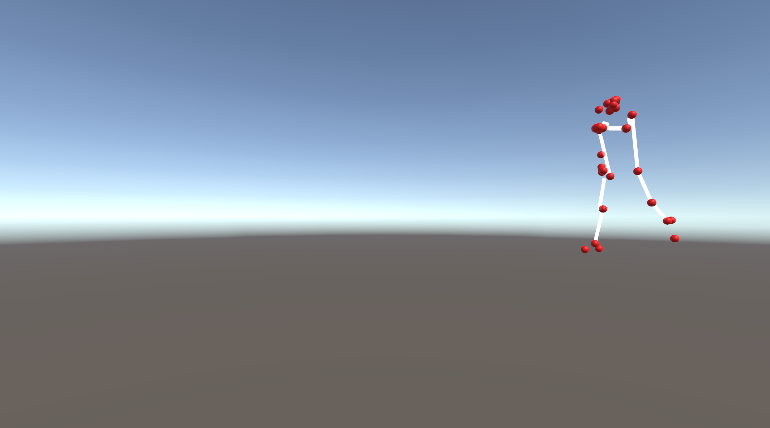
\includegraphics[width=0.4\textwidth]{1}
		\caption{Latent Space\cite{ganlatent}}		
		\label{1}
	\end{figure}
	\FloatBarrier
	Bu nedenle birçok sınıf kullanılarak koşullandırmak anlaşılmasına yardımcı olacaktır.
	Gizli alanda kategori için ortalama bir temsil elde etmek istendiğinde rastgele gizli vektörler kullanılarak onlarca görüntü oluşturulup her kategori için gizli vektörlerin ortalaması alınmalıdır.  
	
	\begin{figure}[h]
		\centering
		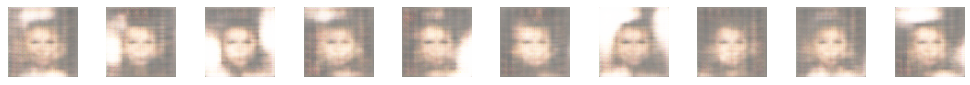
\includegraphics[width=0.4\textwidth]{5}
		\label{5}
		\caption{Koşullandırılmış Latent Space\cite{ganlatent}}
	\end{figure}
	\FloatBarrier
	\subsubsection{GAN'larda Gizli Uzay İnterpolasyonu}
	GAN'larda gizli uzay olarak, Latent Space Interpolation(gizli uzay interpolasyonu) kullanılabilmektedir.
	
	\textbf{Gizli uzay interpolasyonu}, genellikle derin öğrenme modelleri kullanılarak öğrenilen latent (gizli) uzaydaki noktalar arasında doğrusal bir şekilde gezinme veya geçiş yapma sürecidir. Bu, bir model tarafından öğrenilen gizli uzayda, iki farklı nokta arasında doğrusal olarak birbirine yakın noktaların oluşturulması anlamına gelir. Bu işlem, genellikle özellikle görüntü veya ses gibi görsel ve işitsel veri türlerinde etkileyici sonuçlar üretir.
	
	Bu tür interpolasyonlar, yapay zeka alanında yaratıcı uygulamalara olanak tanır. 
	
	Ancak, latent space interpolasyonu yaparken, gizli uzayın doğru bir şekilde öğrenilmesi ve anlamının korunması önemlidir. Aksi halde, interpolasyon sonuçları gerçekçi olmayabilir veya istenmeyen sonuçlar verebilir. Bu nedenle, modelin eğitimi ve latent uzayın analizi önemlidir.
	
	\begin{figure}[h]
		\centering
		\includegraphics[width=0.5\textwidth]{celebalatentspace}
		\label{celebalatentspace}
		\caption{CelebA veri kümesinden iki görüntü arasındaki latent-space interpolation. Orijinal görüntüler her iki tarafta da sunulmaktadır\cite{AutoEncoder-2024-04-04}.}
	\end{figure}
	\FloatBarrier
	İki görüntü arasında geçiş yapmak istediğinizde, gizli uzaydaki görüntüyü oluşturan iki gürültü vektörü arasında doğrusal bir yol üzerinde, oluşturulan iki görüntü gibi bir dizi nokta oluşturulabilir. 
	
	\begin{figure}[h]
		\centering
		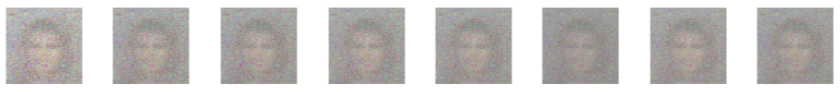
\includegraphics[width=0.35\textwidth]{2}
		\label{2}
		\caption{İki Görüntü Arası Geçiş Yapılarak Oluşturulmuş Görseller\cite{ganlatent}}
	\end{figure}
	\FloatBarrier
	Bu noktalar, oluşturulan iki görüntü arasındaki geçişi gösteren bir dizi görüntü oluşturmak için kullanılabilir. Yani gizli alanda oluşturulan görüntüler kullanılarak yeni görüntüler oluşturulabilir.
	
	\begin{figure}[h]
		\centering
		\includegraphics[width=0.8\textwidth]{interpolasyon}
		\label{interpolasyon}
		\caption{GAN'da Oluşturulan İki Yüz Arasındaki Yoldaki Yüzlere Örnek.\cite{radford2015unsupervised}.}
	\end{figure}
	\FloatBarrier
	Sola bakan ve sağa bakan dört ortalama yüz örneğinden bir "dönüş" vektörü oluşturuldu. Bu vektör, sol ve sağa doğru bakma eylemi arasındaki dönüşü temsil eder. Bu eksen boyunca rastgele örneklere enterpolasyonlar ekleyerek, pozlar güvenilir bir şekilde dönüştürülebildi\cite{radford2015unsupervised}.
	
	\subsubsection{GAN'larda Gizli Uzay Vektör Aritmetiği}
	
	GAN'larda gizli uzayda\textbf{ vektör aritmetiği} denilen bir yön daha vardır. 
	
	Gizli uzay vektörlerini toplayıp çıkarabileceğiniz ve yeni görüntüler üretebileceğiniz anlamına gelmektedir.
	
	\begin{figure}[h]
		\centering
		\includegraphics[width=0.8\textwidth]{vektöraritmetik}
		\label{vektöraritmetik}
		\caption{Latent Space'i anlamak için basit bir vektör aritmetiği örneği\cite{GAN-2024-04-02}.}
	\end{figure}
	\FloatBarrier
	\clearpage
	Yüzleri içeren vektör aritmetiği incelendiğinde örneğin; gülümseyen bir kadının yüzü eksi, nötr bir kadının yüzü artı, tarafsız bir erkeğin yüzü girdileri sonucunda gülümseyen bir adamın yüzü oluşturuldu.
	
	\begin{figure}[h]
		\centering
		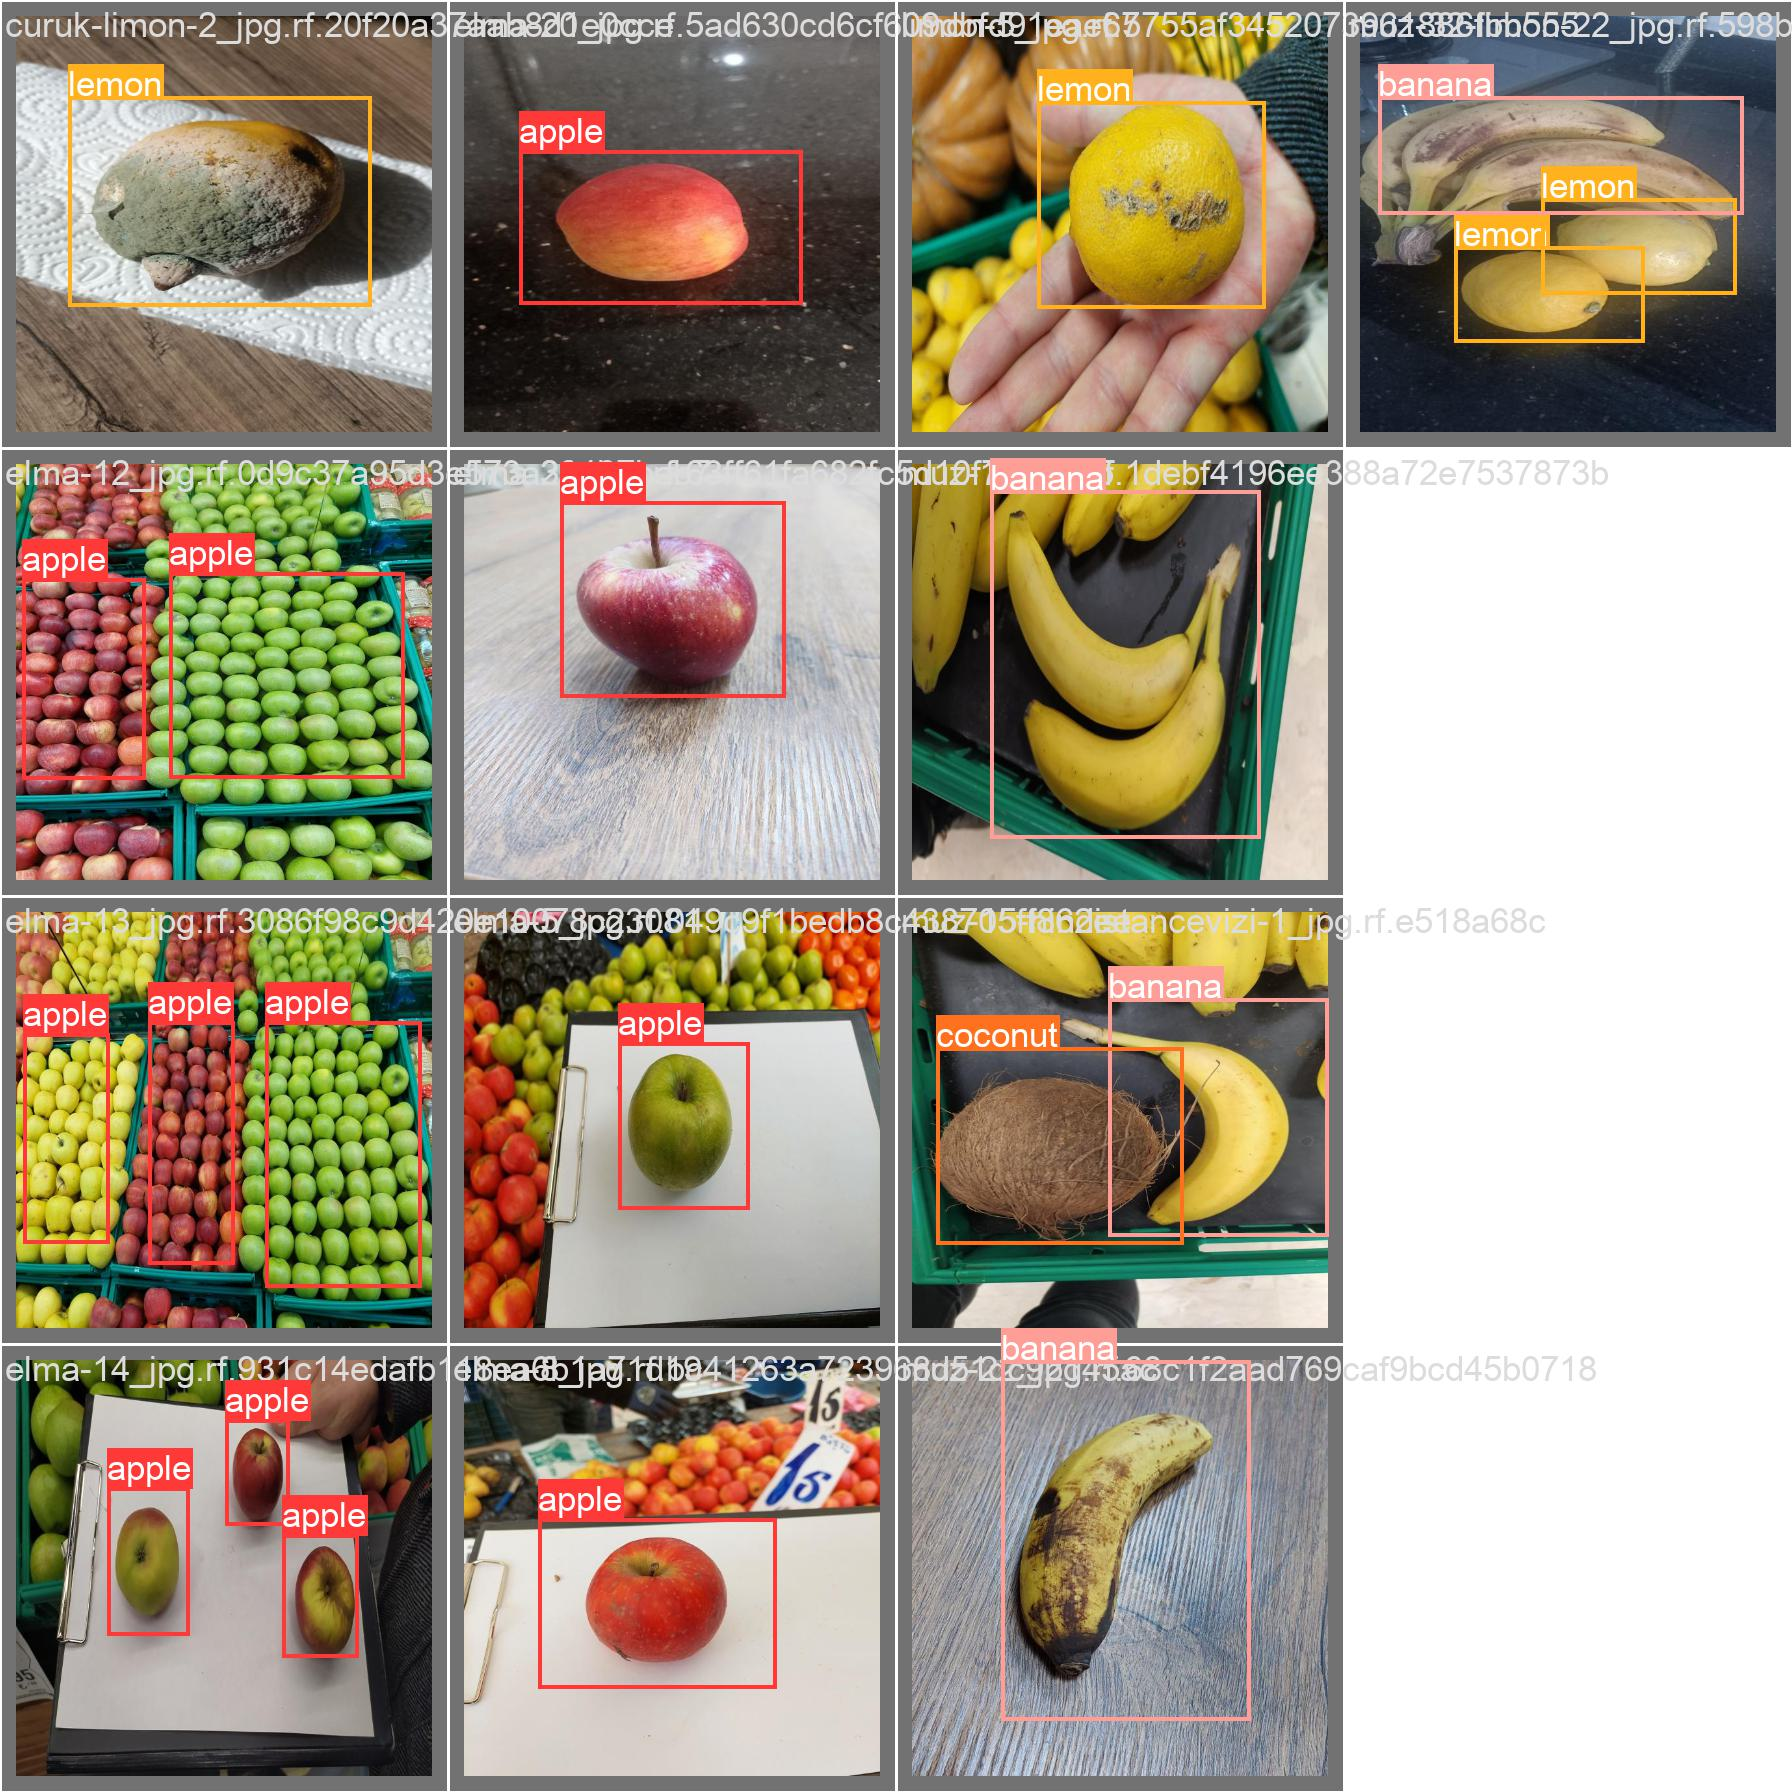
\includegraphics[width=0.9\textwidth]{örnek1}
		\label{örnek1}
		\caption{GAN ile Yüzler Oluşturmak için Gizli Uzaydaki Noktalarda Vektör Aritmetiği Örneği\cite{radford2015unsupervised}}
	\end{figure}
	\FloatBarrier
	\subsubsection{Gizli Alanla İlgili Önemli Noktalar}
	\textbf{Boyutsallığın Azaltılması:} Gizli uzaylar tipik olarak (ancak her zaman değil) orijinal veri uzayından daha düşük bir boyutsallığa sahiptir. Bu boyutluluk azaltma, özellikle karmaşık ve yüksek boyutlu verilerle uğraşırken modelleme sürecini basitleştirmeye ve onu daha takip edilebilir hale getirmeye yardımcı olabilir. 
	
	\textbf{Enterpolasyon ve Manipülasyon:} Gizli alanlar, veriler üzerinde anlamlı manipülasyonlar gerçekleştirme olanağı sunar ve prensip olarak manifoldlarından çıkma riskini önler. Veriler üzerindeki herhangi bir düzenleme işlemi, gizli alandaki uygun bir yörünge açısından anlaşılabilir; bu, belirli niteliklerin değiştirilmesi veya hatta çok daha karmaşık işlemlerin (örneğin kafanın döndürülmesi) gerçekleştirilmesi gibi görevlere izin verir.
	
	\begin{figure}[h]
		\centering
		\includegraphics[width=1\textwidth]{enterpolasyon2}
		\caption{Difüzyon modelinin gizli uzayındaki yörüngeleri takip eden kafa dönüşü.\cite{asperti2023head}.}
		\label{enterpolasyon2}
	\end{figure}
	\FloatBarrier
	Son olarak, gizli uzaydaki noktalar tutulabilir ve basit vektör aritmetiğinde gizli uzayda yeni noktalar oluşturmak için kullanılabilir ve bunlar da görüntüler oluşturmak için kullanılabilir. Bu ilginç bir fikir çünkü görüntülerin sezgisel ve hedefe yönelik oluşturulmasına olanak sağlıyor.
	
	\begin{figure}[h]
		\centering
		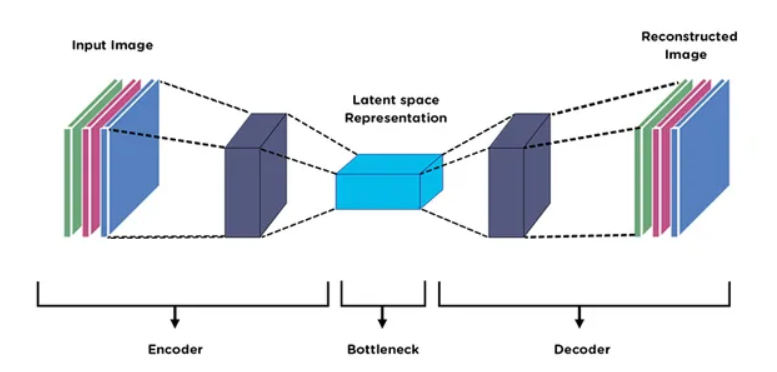
\includegraphics[width=0.9\textwidth]{autoencoder}
		\label{autoencoder}
		\caption{Autoencoder\cite{AutoEncoder-2024-04-04}}
	\end{figure}
	\FloatBarrier
	Soldaki resim MNIST veri setinden alınan gerçek el yazısı rakamlardan oluşuyor. Sağdaki resim ise soldaki resimlerin tam 150 kat sıkıştırılıp tekrar açılmış halini gösteriyor. Bu işlem Autoencoder’lar ile gerçekleştiriliyor.
	
	Latent space'in derin öğrenme uygulamalarındaki önemi, verinin daha basitleştirilmiş bir temsilini oluşturarak veri analizi, öznitelik çıkarma, nesne tanıma, görüntü sentezleme gibi birçok görevde kullanılabilir hale getirmesidir. Ayrıca, bu gizil uzay, benzer veri örneklerini yakın konumlara haritalayarak veri arama ve benzerlik ölçümü gibi işlemlerde de kullanılabilir.
	
	Latent space, genellikle düşük boyutlu olduğu için, verinin daha yüksek boyutlu karmaşık yapısını sıkıştırarak boyutluluk lanetini kırmak anlamına gelir. Bu, daha etkili ve hızlı öğrenme ve çıkarım sağlayabilir. Ancak, latent space'in doğru ve anlamlı bir şekilde öğrenilmesi ve kullanılması önemlidir; aksi halde, veri temsili eksik veya yanıltıcı olabilir.
	\clearpage
	\subsection{GAN Metodu Eğitme}
	\begin{figure}[h]
		\centering
		\includegraphics[width=0.5\textwidth]{genrdisc}
		\label{genrdisc}
		\caption{GAN oluşturma: Oluşturucu-Ayırıcı Çalışma Mantığı\cite{present/youtube/gan/gans_scratch.ipynb-2024-05-01}}
	\end{figure}
	\FloatBarrier
	Oluşturucu rastgele bir tohum vektörünü kabul eder ve bu rastgele vektör tohumundan bir görüntü oluşturur. Ek tohumlar sağlanarak sınırsız sayıda yeni görüntü oluşturulabilir. Ayırıcı, bir görüntüyü girdi olarak kabul eder ve girdi görüntüsünün gerçek olma olasılığı olan sayı üretir.
	
	\subsubsection{Kayıp Fonksiyonları}
	
	Oluşturucu ve ayırıcı birbirine karşı oynamalıdır, yani oluşturucunun ürettiği görüntüler gerçek görüntülere ne kadar yakınsa, ayırıcının onları gerçekten ayırt etmesi o kadar zor olmalıdır. Bu nedenle, kayıp fonksiyonları, bu düşmanca eğitim ortamını sağlamak için tasarlanmalıdır.
	
	Oluşturucu için kayıp fonksiyonu, üretilen görüntülerin ayırıcı tarafından gerçek olarak sınıflandırılmasını amaçlar. Yani oluşturucu, ürettiği görüntülerin ayırıcı tarafından gerçek olarak sınıflandırılmasını sağlamak için eğitilmelidir.
	
	Ayırıcı için kayıp fonksiyonu ise, gerçek görüntülerin 1 ve üretilen görüntülerin 0 olarak sınıflandırılmasını amaçlar. Yani ayırıcı, gerçek ve üretilen görüntüleri doğru şekilde ayırt etmeyi öğrenmelidir\cite{Understanding-2024-05-01},\cite{-2024-05-01}.
	
	Kayıp değerleri, her bir eğitim döneminde (epoch) ağların ne kadar iyi performans gösterdiğini gösterir.
	
	Gen loss (oluşturucu kaybı): Oluşturucunun, ürettiği görüntülerin gerçek görüntülere ne kadar benzediğini ölçer. Daha düşük bir gen kaybı, oluşturucunun daha gerçekçi görüntüler ürettiğini gösterir. Yani, bu değer ne kadar düşükse, oluşturucu o kadar iyi performans gösteriyor demektir.
	
	Disc loss (ayırıcı kaybı): ayırıcı, gerçek ve üretilen görüntüleri doğru şekilde ayırt edip edemediğini ölçer. Daha düşük bir disc kaybı, ayırıcının daha iyi performans gösterdiğini ve gerçek görüntüleri gerçekten ayırt edebildiğini gösterir. Ancak, oluşturucuya karşı adil bir şekilde çalıştığından emin olmak için bu kaybın düşük olması önemlidir\cite{ChatGPT-2024-05-29}.
	
	
	\subsubsection{Ayırıcı'nın Eğitilmesi}
	\begin{figure}[h]
		\centering
		\includegraphics[width=0.7\textwidth]{traindisc}
		\label{genrdisc}
		\caption{Ayırıcı'nın Eğitimi\cite{present/youtube/gan/gans_scratch.ipynb-2024-05-01}}
	\end{figure}
	\FloatBarrier
	Burada eşit sayıda gerçek ve sahte görüntü ile bir eğitim seti oluşturulur. Rastgele tohumlardan eşit sayıda rastgele görüntü üretilir. Ayırıcı eğitim kümesi için X, giriş görüntülerini içerir ve Y, gerçek görüntüler için 1 ve oluşturulanlar için 0 değerini içerir.

	\subsubsection{Oluşturucu'nun Eğitilmesi}
	\begin{figure}[h]
		\centering
		\includegraphics[width=0.7\textwidth]{traingenr}
		\label{genrdisc}
		\caption{Oluşturucu'nun Eğitilmesi\cite{present/youtube/gan/gans_scratch.ipynb-2024-05-01}}
	\end{figure}
	\FloatBarrier
	Oluşturucu eğitim seti için rastgele tohumlar oluştururken, onları eşleştirecek bir etiket vektörüne ihtiyaç duyulmaz ve her zaman 1 değerini içerecek şekilde ayarlanabilir. Bu da oluşturucunun mümkün olan en iyi görüntüleri oluşturmasını ve ayırıcının bu görüntülere yüksek olasılık atamasını sağlar. Çünkü ayırıcı gerçek ve yapay görüntüleri ayırt etmeye çalışırken, bu yapay görüntülerin gerçek görüntülere mümkün olduğunca yakın olmasını ister.
	
	\subsection{StyleGAN-Human}
	
	\begin{figure}[htbp]
		\centering
		\begin{subfigure}{0.18\textwidth}
			\centering
			\includegraphics[width=\textwidth]{startframe}
			\caption{}
			\label{fig:imk1}
		\end{subfigure}
		\hfill
		\begin{subfigure}{0.18\textwidth}
			\centering
			\includegraphics[width=\textwidth]{startframe2}
			\caption{}
			\label{fig:imk2}
		\end{subfigure}
		\hfill
		\begin{subfigure}{0.18\textwidth}
			\centering
			\includegraphics[width=\textwidth]{startframe3}
			\caption{}
			\label{fig:imk3}
		\end{subfigure}
		\\
		\begin{subfigure}{0.18\textwidth}
			\centering
			\includegraphics[width=\textwidth]{startframe4}
			\caption{}
			\label{fig:imk4}
		\end{subfigure}
		\hfill
		\begin{subfigure}{0.18\textwidth}
			\centering
			\includegraphics[width=\textwidth]{startframe5}
			\caption{}
			\label{fig:imk5}
		\end{subfigure}
		\hfill
		\begin{subfigure}{0.18\textwidth}
			\centering
			\includegraphics[width=\textwidth]{endframe}
			\caption{}
			\label{fig:imk6}
		\end{subfigure}
		\caption{Enterpolasyon\cite{fu2022styleganhuman}}
		\label{fig:ssix_images}
		\eqref{fig:imk1}Başlangıç Görseli,
		\eqref{fig:imk2}Akış,
		\eqref{fig:imk3}Akış,
		\eqref{fig:imk4}Akış,
		\eqref{fig:imk5}Akış,
		\eqref{fig:imk6}Son Görsel
	\end{figure}
	\FloatBarrier
	\clearpage
	\begin{figure}[htbp]
		\centering
		\begin{subfigure}{0.35\textwidth}
			\centering
			\includegraphics[width=\textwidth]{sörnek1}
			\caption{}
			\label{fig:ban}
		\end{subfigure}
		\hfill
		\begin{subfigure}{0.35\textwidth}
			\centering
			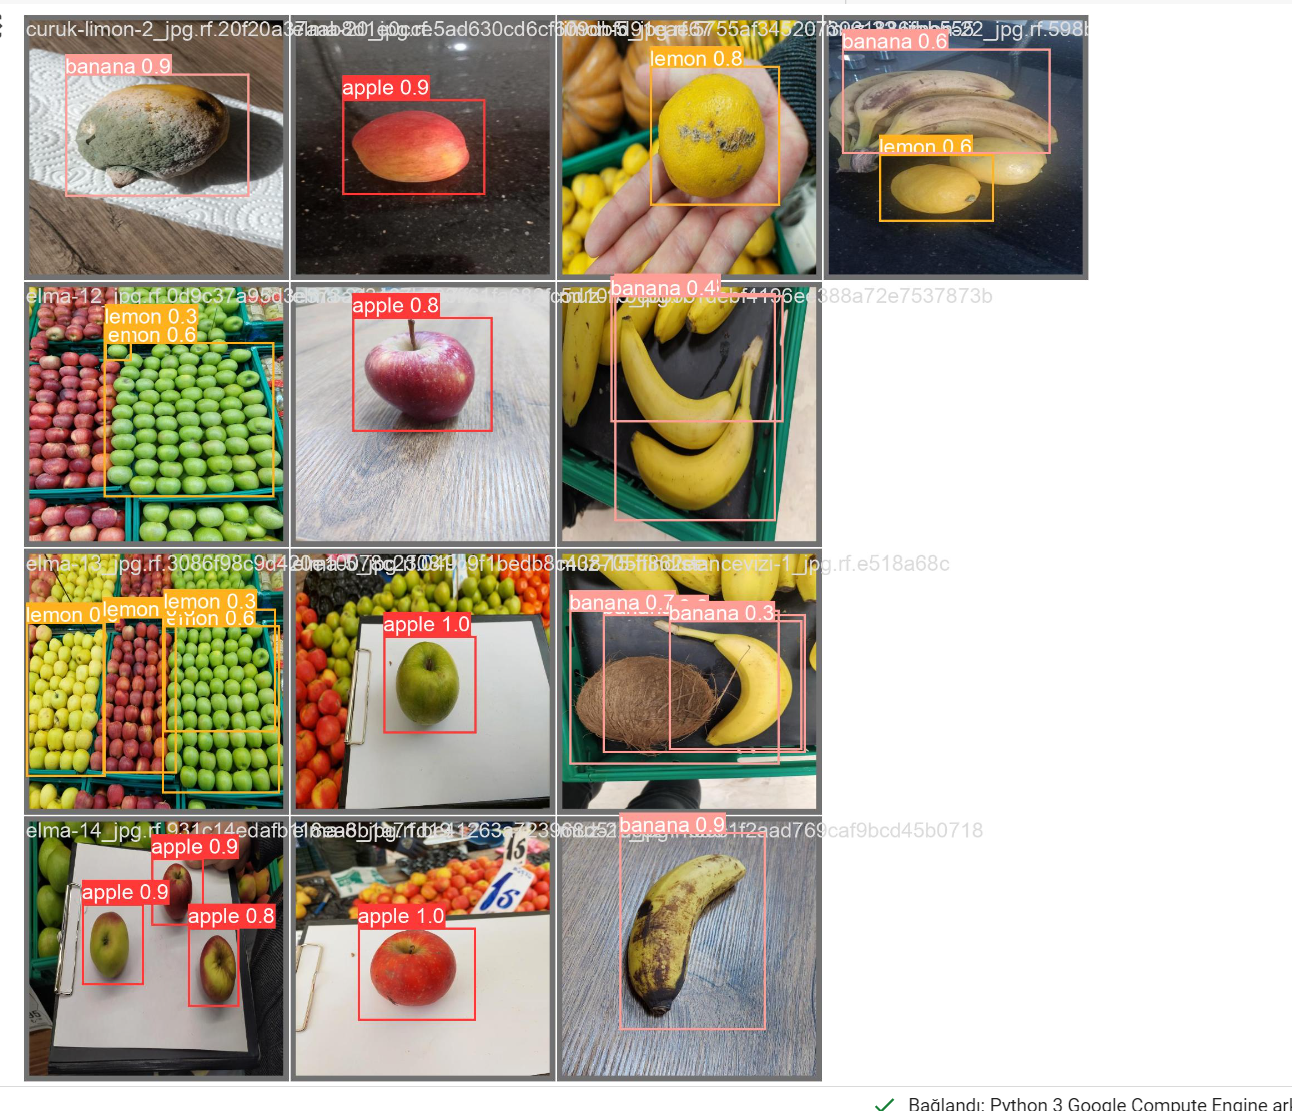
\includegraphics[width=\textwidth]{örnek2}
			\caption{}
			\label{fig:san}
		\end{subfigure}
		\\
		\begin{subfigure}{0.35\textwidth}
			\centering
			\includegraphics[width=\textwidth]{örnek3}
			\caption{}
			\label{fig:kan}
		\end{subfigure}
		\hfill
		\begin{subfigure}{0.35\textwidth}
			\centering
			\includegraphics[width=\textwidth]{örnek4}
			\caption{}
			\label{fig:lan}
		\end{subfigure}
		\caption{Oluşturulan Görsellerle Niteliklerin Düzenlenmesi\cite{fu2022styleganhuman}}
		\eqref{fig:ban},\eqref{fig:san}Üst Uzunluğu Değiştir
		\eqref{fig:kan},\eqref{fig:lan}Alt Uzunluğu Değiştir
	\end{figure}
	\FloatBarrier
	\subsection{Cinsiyet Sınıflandırma}
	Üretilen görüntülerdeki erkek kadın ayırt etmeden üretildiği için cinsiyet sınıflandırma denendi.
	\begin{figure}[h]
		\centering
		\includegraphics[width=0.8\textwidth]{cinssınıf}
		\label{cinssınıf}
		\caption{Cinsiyet Sınıflandırma Kodu-Epoch=10 iken\cite{ChatGPT-2024-05-29}}
	\end{figure}
	
	\begin{figure}[h]
		\centering
		\includegraphics[width=0.7\textwidth]{cinssınıf2}
		\label{cinssınıf2}
		\caption{Cinsiyet Sınıflandırma Kodu-Epoch=10 iken\cite{ChatGPT-2024-05-29}}
	\end{figure}
	
	Bu kodlar eklenip çalıştırıldığında sonuç elde edilemeyen çıktılar aşağıdaki gibidir:
	
	\begin{figure}[htbp]
		\centering
		\begin{subfigure}{0.40\textwidth}
			\centering
			\includegraphics[width=\textwidth]{train-0}
			\caption{}
			\label{fig:ilg1}
		\end{subfigure}
		\hfill
		\begin{subfigure}{0.40\textwidth}
			\centering
			\includegraphics[width=\textwidth]{train-250}
			\caption{}
			\label{fig:ilg2}
		\end{subfigure}
		\\
		\begin{subfigure}{0.40\textwidth}
			\centering
			\includegraphics[width=\textwidth]{train-499}
			\caption{}
			\label{fig:ilg3}
		\end{subfigure}
		\hfill
		\begin{subfigure}{0.40\textwidth}
			\centering
			\includegraphics[width=\textwidth]{train-999}
			\caption{}
			\label{fig:ilg4}
		\end{subfigure}
		\caption{30000 gerçek görüntü ile Sınıflandırma Epoch=10, Görüntü Üretme Epoch=1000 iken 300 gerçek görüntü ile veri setinin eğitilmesi}
		\label{fig:fouur_images}
		\eqref{fig:ilg1}Epoch=0,
		\eqref{fig:ilg2}Epoch=250,
		\eqref{fig:ilg3}Epoch=499,
		\eqref{fig:ilg4}Epoch=999
	\end{figure}
	\FloatBarrier
	
	\begin{figure}[htbp]
		\centering
		\begin{subfigure}{0.40\textwidth}
			\centering
			\includegraphics[width=\textwidth]{epoch10train-0}
			\caption{}
			\label{fig:bam}
		\end{subfigure}
		\hfill
		\begin{subfigure}{0.40\textwidth}
			\centering
			\includegraphics[width=\textwidth]{epoch10train-15}
			\caption{}
			\label{fig:sam}
		\end{subfigure}
		\\
		\begin{subfigure}{0.40\textwidth}
			\centering
			\includegraphics[width=\textwidth]{epoch10train-24}
			\caption{}
			\label{fig:kam}
		\end{subfigure}
		\caption{30000 Sınıflandırma Epoch=10, Görüntü Üretme Epoch=25 iken 30000 gerçek görüntü ile veri setinin eğitilmesi}
		\eqref{fig:bam}Epoch=0,
		\eqref{fig:sam}Epoch=15,
		\eqref{fig:kam}Epoch=24
	\end{figure}
	\FloatBarrier
	
	\clearpage
	\section{Bulgu ve Tartışma}
	
	\subsection{Kod Çıktıları ve Analizler}
	
	\subsubsection{StyleGAN Kod Açıklaması}
	\begin{figure}[h]
		\centering
		\includegraphics[width=0.5\textwidth]{stylegan3gitkod}
		\label{stylegan3gitkod}
		\caption{StyleGAN3 Modelinin Github'tan İndirilmesi\cite{t81_558_deep_learning}}
	\end{figure}
	\FloatBarrier
	\begin{figure}[ht]
		\centering
		\includegraphics[width=0.6\textwidth]{kütüp_generatorkod}
		\label{kütüp_generatorkod}
		\caption{Kütüphanelerin İçe Aktarımı ve Görüntü Fonksiyonları}
	\end{figure} 
	\FloatBarrier
	Stil vektörü, bir yapay sinir ağı modelinin öğrenilen görsel stil özelliklerini temsil eden bir vektördür. Model tarafından öğrenilen görsel stilin ifadesini içerir. Örneğin, dokular, desenler, renk paletleri gibi. StyleGAN'da, stil vektörleri, modelin üretmek istediği görüntünün stil ve özelliklerini kontrol
	eder.
	
	Özellik vektörü, bir yapay sinir ağı modelinin öğrenilen görsel özelliklerini temsil eden bir vektördür. Model tarafından öğrenilen belirli bir özellik veya niteliğin ifadesini içerir. Örneğin, yüz ifadesi, saç rengi, göz rengi, cinsiyet gibi.
	
	Seed2vec fonksiyonu, bir seed parametresi rastgele bir stil vektörü oluşturarak, modelin üreteceği görüntünün stilini belirlemek için bir başlangıç noktası sağlar. Bu stil vektörü, StyleGAN modeli(G) tarafından kullanılarak belirli bir özellik vektörüne sahip bir görüntü oluşturulabilir. Ancak, stil vektörü doğrudan belirli bir özellik vektörünü temsil etmez, sadece görüntünün stilini kontrol etmek için kullanılır.
	
	Fonksiyon, belirli bir seede göre rastgele bir stil vektörü oluşturur ve bu vektörü döndürür.
	
	Görüntüyü ekranda göstermek için kullanılan display\_image fonksiyonu içindeki axis fonksiyonu grafik eksenlerinin görüntü üzerinde gösterilip gösterilmeyeceğini belirler\cite{Matplotlibpyplot.axes-2024-04-17}. 'off' değeri, eksenlerin kapatılacağını ifade eder. Yani, görüntü üzerinde x ve y eksenleri gösterilmeyecek ve görüntü temiz bir şekilde gösterilecektir. Genellikle, yalnızca görüntünün kendisinin odaklanmasını istediğimiz durumlarda eksenler kapatılır.
	
	\begin{figure}[h]
		\centering
		\includegraphics[width=0.7\textwidth]{generatorkod1}
		\label{generatorkod1}
		\caption{Görüntü Oluşturan "generate\_image" Fonksiyonu}
	\end{figure}
	\FloatBarrier

	İlk olarak, \textbf{generate\_image} fonksiyonu, verilen GAN modeli (G), rastgele bir girdi vektörü (z) ve bir kesme parametresi (truncation\_psi) alır. Bu fonksiyon, belirtilen girdi vektörü ve kesme parametresi kullanılarak GAN modeli tarafından bir görüntü oluşturur ve bu görüntüyü döndürür.
	Gs\_kwargs sözlüğü, GAN modelini çalıştırırken kullanılacak argümanları içerir. 
	output\_transform: GAN tarafından üretilen görüntülerin nasıl dönüştürüleceğini belirtir. Bu durumda, tflib.convert\_images\_to\_uint8 işlevi, görüntüleri 0 ile 255 arasındaki tam sayı değerlerine dönüştürür ve nchw\_to\_nhwc parametresi, görüntü dizilimini NCHW'den NHWC'ye dönüştürür.
	
	NCHW: "Batch - Kanal - Yükseklik - Genişlik" anlamına gelir. 
	
	NHWC: "Batch - Yükseklik - Genişlik - Kanal" anlamına gelir\cite{NHWC-2024-04-18}.
	"NCHW'den NHWC'ye dönüştürme" ifadesi, görüntünün piksellerinin düzenini değiştirerek, yükseklik ve genişlik boyutları arasındaki sırayı kanal boyutunun ardına almak anlamına gelir. Bu dönüşüm, farklı derin öğrenme kütüphanelerinin ve modellerin beklediği farklı görüntü dizilimlerini uyumlu hale getirmek için kullanılır.
	
	randomize\_noise: Gürültünün rastgele oluşturulup oluşturulmayacağını belirtir. Bu durumda, gürültü rastgele oluşturulmaz (False)\cite{ChatGPT-2024-05-29}.
	
	truncation\_psi kontrolü: Eğer truncation\_psi değeri None değilse, bu değer Gs\_kwargs sözlüğüne eklenir. truncation\_psi, GAN'ın ürettiği görüntülerin ne kadar kesileceğini belirler. Büyük bir truncation\_psi değeri, daha az kesme anlamına gelir ve daha çeşitli görüntüler elde edilir.
	
	Kesme (truncation), GAN'ların latent uzaydaki (latent space) noktalarından (veya vektörlerinden) görüntüler oluştururken kullanılan bir tekniktir. Bu teknik, GAN'ın öğrendiği dağılımın geniş bir bölgesinden örneklem yapmak yerine, dağılımın daha belirli bir bölgesine odaklanmasını sağlar. Kesme parametresi (truncation parameter), bu kesme işleminin ne kadar yapılacağını kontrol eder. Değer ne kadar büyükse, o kadar az kesme gerçekleşir ve sonuç olarak daha çeşitli, ancak daha az gerçekçi görüntüler elde edilir. Değer ne kadar küçükse, o kadar fazla kesme gerçekleşir ve daha az çeşitli ancak daha gerçekçi görüntüler elde edilir.
	
	Label dizisi, GAN modeline iletilen etiket vektörünü temsil eder. Bu örnek için, etiket vektörü sıfırlardan oluşur ve GAN modelinin giriş boyutlarına uyacak şekilde biçimlendirilir.
	Etiket vektörleri, koşullu GAN'lar gibi bazı GAN modellerinde kullanılan bir kavramdır. Bu modellerde, GAN'ın ürettiği görüntüleri belirli özelliklere göre kontrol etmek veya belirli sınıflara ait görüntüler üretmek isteniyorsa, etiket vektörleri kullanılır. Bu, GAN'ın daha spesifik ve istenen sonuçları üretmesini sağlar. 
	
	G.run(z, label, **G\_kwargs) ifadesi, GAN modelini çalıştırır ve belirtilen girdi vektörü (z) ve etiket (label) kullanılarak bir dizi görüntü oluşturur. Bu fonksiyon, oluşturulan görüntülerin bir listesini döndürür.
	
	\begin{figure}[h]
		\centering
		\includegraphics[width=0.8\textwidth]{getlabelkod}
		\label{getlabelkod}
		\caption{Sınıfa Ait Olacak Etiket Oluşturan "get\_label" Fonksiyonu}
	\end{figure}
	\FloatBarrier
	\textbf{get\_label} fonksiyonu, belirli bir sınıfa ait olacak şekilde etiket oluşturur. Eğer GAN modeli koşullu ise (yani, sınıf bilgisine dayalı olarak görüntü oluşturuyorsa), belirli bir sınıfa ait olduğunu belirtmek için etiketi kullanır. Aksi halde, koşulsuz bir modelde çalışıyorsa etiketi yok sayar.
	
	İlk olarak, torch.zeros fonksiyonuyla, belirtilen boyutlarda (1 satır, GAN modelinin sınıf boyutu kadar sütun) tüm elemanları sıfır olan bir tensor (tensör) oluşturulur. Bu tensor, etiket vektörünü temsil eder. device=device ifadesi, oluşturulan etiket vektörünün belirtilen cihaza gönderilmesini sağlar. Etiket vektörünün cihaza (device) gönderilmesi, PyTorch gibi derin öğrenme çerçevelerinde kullanılan GPU hızlandırması için yapılan bir optimizasyon adımıdır. 
	
	if G.c\_dim != 0: GAN modelinin sınıf boyutu (c\_dim) 0'dan farklıysa, koşullu bir GAN modeli olduğu anlamına gelir. Yani, GAN modeli belirli sınıflara ait görüntüler üretmek için kullanılır.
	
	if class\_idx is None: Eğer sınıf indeksi belirtilmemişse (None olarak atanmışsa), bir hata mesajı gösterilir. Çünkü koşullu bir GAN modelinde, belirli bir sınıfa ait bir görüntü üretmek için sınıf indeksi belirtilmelidir.
	
	label[:, class\_idx] = 1: Eğer sınıf indeksi belirtilmişse, ilgili indekse sahip eleman 1 olarak atanır. Bu, etiket vektöründe belirtilen sınıfa ait olduğunu gösterir. Örneğin, eğer sınıf indeksi 2 ise, etiket vektörünün 2. indeksine 1 atanır.
	
	else: GAN modelinin sınıf boyutu 0 ise, koşulsuz bir GAN modeli olduğu anlamına gelir. Yani, üretilecek görüntüler belirli bir sınıfa ait olmadan üretilecektir.
	
	if class\_idx is not None: Eğer sınıf indeksi belirtilmişse (None değilse), ancak model koşulsuz bir modelse, bir uyarı mesajı gösterilir. Çünkü sınıf indeksi belirtmenin bir anlamı yoktur, çünkü model koşullu olmadığı için sınıflar arasında ayrım yapılmaz.
	
	return label: Son olarak, oluşturulan etiket vektörü döndürülür. Bu vektör, GAN modelinin koşullu olup olmadığına bağlı olarak belirli bir sınıfa ait olup olmadığını belirtir veya koşulsuz bir modelse sınıf bilgisi içermez.
	
	\begin{figure}[h]
		\centering
		\includegraphics[width=1\textwidth]{generatorkod2}
		\label{generatorkod2}
		\caption{Daha Fazla Kontrol Sağlayarak Görüntü Oluşturan "generate\_image" Fonksiyonu}
	\end{figure}
	\FloatBarrier
	\textbf{generate\_image} fonksiyonu, belirli bir cihazda (GPU veya CPU), bir GAN modeli (G), bir girdi vektörü (z), bir kesme parametresi (truncation\_psi), bir gürültü modu (noise\_mode) ve bir sınıf indeksi (class\_idx) alır. Bu parametrelerle birlikte, bu fonksiyon, GAN modelini kullanarak bir görüntü oluşturur ve bu görüntüyü döndürür.
	
	Kodda iki ayrı generate\_image fonksiyonu tanımlanmış, her biri farklı kullanım senaryolarına yönelik olarak tasarlanmıştır. İlk fonksiyon GAN modelini kullanarak bir görüntü oluşturur. İkinci fonksiyonda aynı şekilde GAN modelini kullanarak bir görüntü oluşturur, ancak bu sefer daha fazla kontrol sağlar. Örneğin, belirli bir cihazda çalıştırma, gürültü modunu belirleme ve koşullu GAN kullanma gibi. İhtiyaca göre hangi fonksiyonun kullanılacağına karar verilebilir.
	
	z=torch.from\_numpy(z).to(device): Girdi vektörü (z), bir NumPy dizisinden bir PyTorch tensorüne dönüştürülür ve belirtilen cihaza (device) gönderilir. PyTorch tensorleri, genellikle modelin ve verinin saklandığı ve işlendiği veri yapısıdır.
	Girdi verisini PyTorch tensorüne dönüştürmek, derin öğrenme modellerini eğitmek ve çıkarım yapmak için gereken uyumluluk, optimize edilmiş işlemler ve paralel işleme yeteneklerinden yararlanmak için yapılır.
	
	label = get\_label(G, device, class\_idx): Belirli bir GAN modeli (G), bir cihaz (device) ve bir sınıf indeksi (class\_idx) alır ve bu bilgilere dayanarak bir etiket vektörü oluşturur.
	
	img = G(z, label, truncation\_psi=truncation\_psi, noise\_mode=noise\_mode): Oluşturulan girdi vektörü (z) ve etiket vektörü (label), GAN modeli (G) tarafından kullanılarak bir görüntü oluşturulur. Bu işlem, GAN modelinin çağrılmasıyla gerçekleşir. Kesme parametresi (truncation\_psi) ve gürültü modu (noise\_mode) belirtilen değerlerle iletilir.
	
	img = (img.permute(0, 2, 3, 1) * 127.5 + 128).clamp(0, 255).to(torch.uint8): Oluşturulan görüntü, uygun formatta işlenir. Öncelikle, görüntünün boyutları değiştirilir ve renk kanallarının sırası ayarlanır (PyTorch'da varsayılan olarak NCHW, bu işlem NHWC'ye dönüştürür). Daha sonra, piksel değerleri uygun bir şekilde ölçeklenir ve sınırlanır, ardından piksel değerleri tam sayı tipine dönüştürülür.
	
	return PIL.Image.fromarray(img[0].cpu().numpy(), 'RGB'): Oluşturulan görüntü, PIL (Python Imaging Library) kütüphanesinin Image.fromarray fonksiyonu kullanılarak bir PIL görüntü nesnesine dönüştürülür ve bu nesne döndürülür. Bu adım, oluşturulan görüntünün dışarı aktarılabilir bir formata dönüştürülmesini sağlar.
	
	\begin{figure}[h]
		\centering
		\includegraphics[width=1\textwidth]{urlkod}
		\label{urlkod}
		\caption{Önceden Eğitilmiş Veri Setini İndirme}
	\end{figure}
	\FloatBarrier
	Bu URL, NGC(NVIDIA GPU Cloud) API'sine\cite{NVIDIA-2024-04-18} istek göndererek belirli bir model dosyasını indirmek için kullanılacaktır. NGC, NVIDIA'nın bulut tabanlı hizmetidir ve yapay zeka, derin öğrenme ve HPC (yüksek performanslı hesaplama) alanlarında kullanılan yazılım, araçlar ve modellerin barındırılmasını ve dağıtılmasını sağlar.
	
	StyleGAN2 modelini indirir ve yükler, böylece bu model daha sonra görüntü üretimi için kullanılabilir hale gelir.
	
	Kullanıcıya, indirilecek modelin URL'sinin yüklenmeye başlandığına dair bir mesaj gösterilir.
	
	PyTorch'da, modelin işleneceği cihaz belirlenir. 'cuda', yani GPU, belirlenen cihazdır. Bu, modelin GPU üzerinde çalışacağı anlamına gelir.
	
	Dnnlib kütüphanesi tarafından sağlanan open\_url fonksiyonu, belirtilen URL'den bir dosya açar ve bu dosyayı 'f' adıyla kullanılabilir hale getirir. 'with' ifadesi, dosyanın kullanımı bittiğinde otomatik olarak kapatılmasını sağlar.
	
	NGC API'sinden indirilen dosya, 'load\_network\_pkl' fonksiyonu kullanılarak yüklenir. Bu fonksiyon, StyleGAN2 modelinin ağırlıklarını içeren bir sözlük döndürür. 'G\_ema', eğitim sırasında kullanılan bir model üstel hareketli ortalamasıdır ve genelde daha iyi sonuçlar verir. 'to(device)' ifadesi, yüklenen modelin belirtilen cihaza (GPU) taşınmasını sağlar.
	
	Hareketli ortalama, bir zaman serisi verisinin belirli bir zaman aralığındaki ortalamasını alır ve bu ortalama değeri belirli bir katsayı ile ağırlıklandırır. Üstel Hareketli Ortalama (Exponential Moving Average, EMA) ise standart hareketli ortalama yöntemlerinden biridir.
	
	EMA, daha yakın zaman dilimlerine daha fazla ağırlık vererek son zamanlardaki verilere daha fazla önem atfeder. Bu, yeni veriler geldikçe ortalama değerinin hızlı bir şekilde güncellenmesini sağlar.
	
	\begin{equation}
		EMA_t = \alpha \times X_t + (1-\alpha) \times EMA_{t-1}
		\label{EMA}
	\end{equation}
	
	Formül \eqref{EMA}'de Üstel Hareketli Ortalamanın Genel Formülü Verilmiştir\cite{ChatGPT-2024-05-29}.
	
	$EMA_t$ mevcut zaman $t$'ye ait EMA değeridir, 
	
	$X_t$ mevcut zaman $t$'ye ait veri değeridir,
	
	$\alpha$ bir düzeltme faktörüdür ve genellikle 0 ile 1 arasında bir değer alır. Bu değer, yeni verilere ne kadar ağırlık verileceğini belirler.
	
	\begin{figure}[h]
		\centering
		\includegraphics[width=1\textwidth]{imagekod}
		\label{imagekod}
		\caption{Görüntü Oluşturma ve Görsel Olarak İnceleme}
	\end{figure}
	\FloatBarrier

	Belirli bir GAN modeli kullanılarak belirli bir seed aralığındaki görüntülerin oluşturulmasını ve görsel olarak incelenmesini sağlar.
	
	SEED\_FROM = 1000 ve SEED\_TO = 1015: Oluşturulacak görüntülerin seed aralığı belirlenir. SEED\_FROM, oluşturulacak görüntülerin seedlerinin başlangıç değerini, SEED\_TO ise son değerini belirtir.
	
	for i in range(SEED\_FROM, SEED\_TO): Belirtilen seed aralığında bir döngü başlatılır. Bu döngü, seed aralığındaki her bir değer için görüntü oluşturulmasını sağlar.
	
	print(f"Seed {i}"): Her bir seed değeri için bir başlık yazdırılır. Bu, hangi seed değeri ile oluşturulan görüntünün ekranda gösterildiğini belirtir.
	
	z = seed2vec(G, i): Her bir seed değeri için, seed2vec fonksiyonu kullanılarak bir latent vektör (z) oluşturulur. Bu latent vektör, GAN modeline verilerek görüntü oluşturulmasını sağlar.
	
	img = generate\_image(device, G, z): Oluşturulan latent vektör (z) ve GAN modeli (G) kullanılarak görüntü oluşturulur. generate\_image fonksiyonu, verilen latent vektörü ve modeli kullanarak bir görüntü döndürür.
	
	display\_image(img): Oluşturulan görüntü ekranda gösterilir. Bu, her bir seed değeri için oluşturulan görüntülerin görsel olarak incelenmesini sağlar.

	\subsubsection{StyleGAN3 Modeli Kod Çıktı Örnekleri}
	
	\begin{figure}[htbp]
		\centering
		\begin{subfigure}{0.34\textwidth}
			\centering
			\includegraphics[width=\textwidth]{çıktı1}
			\caption{}
			\label{fig:emg1}
		\end{subfigure}
		\hfill
		\begin{subfigure}{0.34\textwidth}
			\centering
			\includegraphics[width=\textwidth]{çıktı2}
			\caption{}
			\label{fig:emg2}
		\end{subfigure}
		\\
		\begin{subfigure}{0.34\textwidth}
			\centering
			\includegraphics[width=\textwidth]{çıktı4}
			\caption{}
			\label{fig:emg3}
		\end{subfigure}
		\hfill
		\begin{subfigure}{0.34\textwidth}
			\centering
			\includegraphics[width=\textwidth]{çıktı3}
			\caption{}
			\label{fig:emg4}
		\end{subfigure}
		\caption{StyleGAN3 Modelinde CelebA-HQ Veri Setiyle Oluşturulan Sahte Yüz Örnekleri}
		\label{fig:fourr_images}
	\end{figure}
	\FloatBarrier
	\clearpage
	\subsubsection{DCGAN Modeli Kod Çıktıları}
	
	\begin{figure}[htbp]
		\centering
		\begin{subfigure}{0.40\textwidth}
			\centering
			\includegraphics[width=\textwidth]{300epoch50train-0}
			\caption{}
			\label{fig:han}
		\end{subfigure}
		\hfill
		\begin{subfigure}{0.40\textwidth}
			\centering
			\includegraphics[width=\textwidth]{300epoch50train-49}
			\caption{}
			\label{fig:man}
		\end{subfigure}
		\caption{Epoch=50 iken 300 gerçek görüntü ile veri setinin eğitilmesi}
		\eqref{fig:han}Epoch=0,
		\eqref{fig:man}Epoch=49
	\end{figure}
	\FloatBarrier
	\begin{figure}[htbp]
		\centering
		\begin{subfigure}{0.45\textwidth}
			\centering
			\includegraphics[width=\textwidth]{300epoch100train-0}
			\caption{}
			\label{fig:ian}
		\end{subfigure}
		\hfill
		\begin{subfigure}{0.45\textwidth}
			\centering
			\includegraphics[width=\textwidth]{300epoch100train-49}
			\caption{}
			\label{fig:aan}
		\end{subfigure}
		\\
		\begin{subfigure}{0.45\textwidth}
			\centering
			\includegraphics[width=\textwidth]{300epoch100train-99}
			\caption{}
			\label{fig:ean}
		\end{subfigure}
		\caption{Epoch=100 iken 300 gerçek görüntü ile veri setinin eğitilmesi}
		\eqref{fig:ian}Epoch=0,
		\eqref{fig:aan}Epoch=49,
		\eqref{fig:ean}Epoch=99
	\end{figure}
	
	\begin{figure}[htbp]
		\centering
		\begin{subfigure}{0.45\textwidth}
			\centering
			\includegraphics[width=\textwidth]{300epoch1000train-0}
			\caption{}
			\label{fig:1000e0}
		\end{subfigure}
		\hfill
		\begin{subfigure}{0.45\textwidth}
			\centering
			\includegraphics[width=\textwidth]{300epoch1000train-500}
			\caption{}
			\label{fig:1000e499}
		\end{subfigure}
		\\
		\begin{subfigure}{0.45\textwidth}
			\centering
			\includegraphics[width=\textwidth]{300epoch1000train-999}
			\caption{}
			\label{fig:1000e999}
		\end{subfigure}
		\caption{Epoch=1000 iken 300 gerçek görüntü ile veri setinin eğitilmesi}
		\eqref{fig:1000e0}Epoch=0,
		\eqref{fig:1000e499}Epoch=499,
		\eqref{fig:1000e999}Epoch=999
	\end{figure}
	
	\begin{figure}[htbp]
		\centering
		\begin{subfigure}{0.45\textwidth}
			\centering
			\includegraphics[width=\textwidth]{30000epochtrain-0}
			\caption{}
			\label{fig:ing1}
		\end{subfigure}
		\hfill
		\begin{subfigure}{0.45\textwidth}
			\centering
			\includegraphics[width=\textwidth]{30000epochtrain-24}
			\caption{}
			\label{fig:ing2}
		\end{subfigure}
		\\
		\begin{subfigure}{0.45\textwidth}
			\centering
			\includegraphics[width=\textwidth]{30000epochtrain-49}
			\caption{}
			\label{fig:ing3}
		\end{subfigure}
		\caption{Epoch=50 iken 30000 gerçek görüntü ile veri setinin eğitilmesi}
		\eqref{fig:ing1}Epoch=0,
		\eqref{fig:ing2}Epoch=24,
		\eqref{fig:ing3}Epoch=49
	\end{figure}
	\begin{figure}[htbp]
		\centering
		\begin{subfigure}{0.48\textwidth}
			\centering
			\includegraphics[width=\textwidth]{30000epoch100train-0}
			\caption{}
			\label{fig:30000e100-0}
		\end{subfigure}
		\hfill
		\begin{subfigure}{0.48\textwidth}
			\centering
			\includegraphics[width=\textwidth]{30000epoch100train-78}
			\caption{}
			\label{fig:30000e100-78}
		\end{subfigure}
		\caption{Epoch=100 iken 30000 gerçek görüntü ile veri setinin eğitilmesi}
		\eqref{fig:30000e100-0}Epoch=0,
		\eqref{fig:30000e100-78}Epoch=78,
	\end{figure}
	\FloatBarrier
	
	Bu verilerden bir çıkarım yapılırsa daha fazla veri girdisi daha gerçekçi daha net ve en temel sonuç olarak daha iyi eğitilmiş örnekler verir. Epoch sayısı arttıkça gelişim ve çeşitlilik de artarken veri girdisi arttıkça bu sonuç daha net gözüküyor.
	
	\subsubsection{CGAN Modeli Kod Çıktıları}
	
	Başlangıç mimarisiyle oluşturulan görüntüler bulanıktı, konturlar iyi tanımlanmamıştı ve yalnızca erkek/kadın gibi çok ayırıcı etiketlerle çalışılıyordu. Çıktı yalnızca gürültüden ibaretti. 
	
	\begin{figure}[htbp]
		\centering
		\begin{subfigure}{0.48\textwidth}
			\centering
			\includegraphics[width=\textwidth]{startepoch1}
			\caption{}
			\label{fig:ima1}
		\end{subfigure}
		\hfill
		\begin{subfigure}{0.48\textwidth}
			\centering
			\includegraphics[width=\textwidth]{startepoch5}
			\caption{}
			\label{fig:ima2}
		\end{subfigure}
		\caption{Başlangıç Mimarisi(202.599 veri kullanıldı.)\cite{fu2022styleganhuman}}
		\label{fig:siix_images}
		\eqref{fig:ima1}Epoch=0,
		\eqref{fig:ima2}Epoch=5,
	\end{figure}
	\FloatBarrier
	\clearpage
	Bazı ek özelliklerle birlikte tek sıcak kodlamayı kullanan hem oluşturucuda hem de ayırıcıda birden fazla etiket kullanacak şekilde değiştirilmiş temel mimaridir. 
	Bir sıcak kodlama (OHE), kategorik verileri sayısal olanlara kodlayan bir tekniktir\cite{Tek-2024-05-14}.
	
	\begin{figure}[htbp]
		\centering
		\begin{subfigure}{0.38\textwidth}
			\centering
			\includegraphics[width=\textwidth]{finalepoch1}
			\caption{}
			\label{fig:im1}
		\end{subfigure}
		\hfill
		\begin{subfigure}{0.38\textwidth}
			\centering
			\includegraphics[width=\textwidth]{finalepoch11}
			\caption{}
			\label{fig:im2}
		\end{subfigure}
		\caption{Final Mimarisi(202.599 veri kullanıldı.)\cite{fu2022styleganhuman}}
		\label{fig:six_images}
		\eqref{fig:im1}Epoch=0,
		\eqref{fig:im2}Epoch=11,
	\end{figure}
	\FloatBarrier
	İlk adımda, MyCustomDataset sınıfı, veri kümesini yükler. Bu sınıf, belirtilen etiket sütunlarını okuyarak ve görüntüleri uygun şekilde işleyerek veri kümesini hazırlar.
	
	Generator sınıfı, girdi olarak alınan rastgele bir gürültü vektörüne (latent vektör) ve etiketlere dayanarak (örneğin, cinsiyet ve saç rengi) görüntüleri üretir. Kadın ve erkek yüzlerinin ayrı ayrı üretilmesi için bu etiketler kullanılır. Özellikle, forward yöntemi, gürültü ve etiketleri alır ve uygun katmanları geçerek sonunda bir görüntü üretir.
	
	Sonuç olarak final mimarisinin sonuçlarının başlangıç mimarisine göre daha yüksek çözünürlüklü ve daha gerçekçi görüntüler ürettiği anlaşılmıştır.
	
	\subsubsection{CycleGAN Modeli Kod Çıktıları}
	CycleGAN, bir görüntü sınıfının stilini başka bir görüntü sınıfının stiline veya tam tersi şekilde aktarmayı amaçlayan bir model mimaridir. Bu örnekte gülümsemeyen bir yüzü gülümseyen bir yüze çevirmek amaçlanmıştır.
	\begin{figure}[h]
		\centering
		\includegraphics[width=0.38\textwidth]{indir}
		\label{indir}
		\caption{CycleGAN Örneği. Epoch=20\cite{Introduction-2024-05-22}}
	\end{figure}
	\clearpage
	
	\begin{figure}[h]
		\centering
		\includegraphics[width=0.5\textwidth]{epoch50}
		\label{epoch50}
		\caption{CycleGAN Örneği. Epoch=50\cite{Introduction-2024-05-22}}
	\end{figure}	
	\clearpage
	
	\begin{figure}[h]
		\centering
		\includegraphics[width=0.5\textwidth]{epoch100}
		\label{epoch100}
		\caption{CycleGAN Örneği. Epoch=100\cite{Introduction-2024-05-22}}
	\end{figure}
	
	
	\FloatBarrier
	
	\clearpage
	\subsubsection{Steps-Per-Epoch Eklenmiş Kod Çıktıları}
	
	\begin{figure}[h]
		\centering
		\includegraphics[width=0.38\textwidth]{stepperepoch100}
		\label{stepperepoch100}
		\caption{Epoch=10, Steps-Per-Epoch=100 CycleGAN Örneği }
	\end{figure}	
	\FloatBarrier
	\clearpage
	
	\begin{figure}[h]
		\centering
		\includegraphics[width=0.5\textwidth]{stepperepoch1002}
		\label{stepperepoch1002}
		\caption{Epoch=20, Steps-Per-Epoch=100 CycleGAN Örneği }
	\end{figure}	
	\clearpage
	
	\begin{figure}[h]
		\centering
		\includegraphics[width=0.5\textwidth]{stepperepoch500}
		\label{stepperepoch500}
		\caption{Epoch=5, Steps-Per-Epoch=500 CycleGAN Örneği}
	\end{figure}	
	\FloatBarrier
	\clearpage
	\subsubsection{Steps-Per-Epoch İçin Eklenen Kod}
	\begin{figure}[h]
		\centering
		\includegraphics[width=1\textwidth]{spekod}
		\label{spekod}
		\caption{Steps-Per-Epoch Kodu\cite{ChatGPT-2024-05-29}}
	\end{figure}	
	\FloatBarrier
	\subsection{Gülümseme Algılama}
	Buradaki amaç GAN metodu ile yüz rastgele yüzler üretip bu üretilen görüntülerdeki gülümseme algılama uygulaması yapmaktı. 
	
	\begin{figure}[h]
		\centering
		\includegraphics[width=0.5\textwidth]{deneme}
		\label{deneme}
		\caption{Celeb-A Veri Setini Kullanarak Gülümseme Algılama\cite{Smile-Detection}}
	\end{figure}	
	\FloatBarrier
	\clearpage
	\subsection{Karşılaşılan Hatalar}
	
	\begin{figure}[h]
		\centering
		\includegraphics[width=0.8\textwidth]{GPUbeyaz}
		\label{GPUbeyaz}
		\caption{"Sisteminizde Hiçbir NVIDIA Sürücüsü Bulunamadı" Hatası}
	\end{figure}
	\FloatBarrier
	Bu hatanın sebebi Colab Notebook ayarlarından donanım hızlandırıcı seçeneğinden GPU'yu seçmemek, yani bağlantıyı GPU üzerinden yapmamaktır. Bu hatanın çözümü Colab Notebook ayarlarından donanım hızlandırıcı olarak T4 GPU seçilip, bağlantıyı yeniden kurmak ve tüm kodları tekrar çalıştırmaktır.
	\subsubsection{StyleGAN3 Kodunda Alınan Hatalar}
	StyleGan3 modelinde önceden eğitilmiş\cite{StyleGAN3-2024-04-16} CelebA-HQ veri seti olmadığından StyleGan2 modelinde önceden eğitilmiş\cite{StyleGAN2-2024-04-14} CelebA-HQ veri setinin 256x256 çözünürlüklü bir veri setini bulundu ve denendi. Sonuç gayet başarılıydı. Ancak hedef 1028x1028 çözünürlüklü veri setiyle yapabilmek ve dosyaları drive'dan çekmeye çalışmaktı ama şu an StyleGan3 modeline aktarmada sıkıntı yaşandı ve hata alındı.
	
	\begin{figure}[h]
		\centering
		\includegraphics[width=0.5\textwidth]{picklehata}
		\label{picklehata}
		\caption{"'tuple' object does not support item assignment" Hatası}
	\end{figure}
	\FloatBarrier
	Çözüm olarak legacy.py dosyası tekrar yüklendi ve incelendi ancak hata çözülemedi. 
	
	\begin{figure}[ht]
		\centering
		\includegraphics[width=0.7\textwidth]{zdim}
		\label{zdim}
		\caption{"Cannot convert '100' to a shape." Hatası}
	\end{figure}
	\FloatBarrier
	Bu hatanın sebebi, input katmanındaki shape parametresinin beklediği değerin bir tuple (dizi) olması gerektiği halde, doğrudan bir sayı olan 100 değerinin verilmiş olmasıdır.
	Bu hatanın çözümü ise 100 değerinin değişkeni olan z\_dim'in bulunduğu shape=(z\_dim) satırını shape=(z\_dim,) olarak değiştirip bu kod satırını tekrar çalıştırmaktır.
	
	Bir sinir ağı, giriş verisini alırken, genellikle bu verinin boyutunu bilmek ister. Örneğin, bir resim sınıflandırma modeli düşünelim. Bu model, resimlerin piksel değerlerini alır ve her bir pikseli ayrı bir özellik olarak düşünür. Dolayısıyla, giriş verisinin boyutu, resmin genişliği, yüksekliği ve kanal sayısına bağlı olacaktır.
	
	Ancak, bu boyut tek bir sayı olarak ifade edilmez. Örneğin, bir renkli resim için, boyut (genişlik, yükseklik, kanal sayısı) şeklinde bir dizi olabilir: (genişlik, yükseklik, kanal). Bu dizi, resmin boyutunu tam olarak tanımlar.
	
	Benzer şekilde, sinir ağlarında, giriş katmanının shape parametresi de bir dizi şeklinde beklenir. Eğer sadece bir sayı verilirse, bu sadece tek bir boyutlu bir veri olduğunu belirtir. Ancak, tipik olarak, daha karmaşık verilerin boyutları daha fazla boyut içerecek şekilde olur.
	
	Burada, z\_dim olarak adlandırılan bir değişken var. Bu genellikle bir gizli katmanın boyutunu veya latent uzayın boyutunu temsil eder. Dolayısıyla, bu boyutu input katmanının shape parametresine geçirerek, sinir ağının giriş boyutunu belirlemiş oluyorsunuz.
	
	Sonuç olarak, shape=(z\_dim,) olarak ayarlamak, input katmanının beklediği şekil parametresini doğru formatta sağlayarak hatayı çözer. Bu, sinir ağının giriş verisinin beklenen boyuta ve yapıya sahip olduğunu belirtir.
	\clearpage
	\subsubsection{CGAN Kodunda Alınan Hatalar}
	\begin{figure}[h]
		\centering
		\includegraphics[width=0.7\textwidth]{tensorboardhata}
		\label{tensorboardhata}
		\caption{"No module named 'tensorboardcolab'" Hatası\cite{SZamboni-CGANCelebA-2024-05-13}}
	\end{figure}
	\FloatBarrier
	Kodda alınan hata aşağıdaki kod parçasıyla çözüldü.
	
	\begin{figure}[h]
		\centering
		\includegraphics[width=1\textwidth]{tensorboardcozum}
		\label{tensorboardcozum}
		\caption{"No module named 'tensorboardcolab'" Hatasının Çözüm Kodu\cite{SZamboni-CGANCelebA-2024-05-13}}
	\end{figure}
	\FloatBarrier
	Bu hatanın çözümünün ardından aşağıdaki hata ile karşılaşıldı.
	
	\begin{figure}[h]
		\centering
		\includegraphics[width=0.6\textwidth]{waitforhata}
		\label{waitforhata}
		\caption{"Initialization failed, retry again" Hatası\cite{SZamboni-CGANCelebA-2024-05-13}}
	\end{figure}
	\FloatBarrier
	Bu hatanın çözümü kodda "Tensorboard" kullanmayarak çözüldü\cite{ChatGPT-2024-05-29}. Tensorboard kullanılmayan kod aşağıda verilmiştir.
	\FloatBarrier
	\clearpage
	
	\begin{lstlisting}[language=Python, breaklines=true, breakatwhitespace=true, basicstyle=\ttfamily, columns=fullflexible]
def main():
device = torch.device("cuda:0" if (torch.cuda.is\_available() and ngpu > 0) else "cpu")
print("Use device: " + str(device))

# Load data
data\_loader = getDataLoader(input\_dir, batch\_size, image\_size, num\_workers, labels\_number)

# Save a sample of the training data
show\_images = next(iter(data\_loader))
plt.imshow(np.transpose(vutils.make\_grid(show\_images[0][0:64], padding=2, normalize=True), (1, 2, 0)))
plt.savefig(str(output\_dir) + 'training\_sample' + '.png')

# Create the Generator
netG = Generator().to(device)
print(netG)

# Create the Discriminator
netD = Discriminator().to(device)
print(netD)

# Set the cost function
cost\_fun = nn.BCELoss()

real\_label = 1.0  # Change to float
fake\_label = 0.0  # Change to float

# Create Discriminator and Generator optimizer
optimizerD = optim.Adam(netD.parameters(), lr=lr, betas=(beta1, 0.999))
optimizerG = optim.Adam(netG.parameters(), lr=lr, betas=(beta1, 0.999))

# Start training
for current\_epoch in range(num\_epochs):
	for batch\_index, (data, lbl) in enumerate(data\_loader, 0):
		# Encode real labels for the discriminator
		lbl\_real\_disc = getDiscriminatorLabels(lbl, batch\_size, image\_size)
		
		# Reset discriminator gradients
		netD.zero\_grad()
		
		# Train discriminator on real data
		real\_data = data.to(device)
		lbl\_real\_disc = lbl\_real\_disc.to(device)
		b\_size = real\_data.size(0)
		targets = torch.full((b\_size,), real\_label, device=device)
		outputs = netD(real\_data, lbl\_real\_disc).view(-1)
		real\_loss = cost\_fun(outputs, targets)
		real\_loss.backward()
		D\_x = outputs.mean().item()
		
		# Generate fake data
		fake\_in\_lbl\_clear = np.random.randint(2, size=(batch\_size, n\_labels))
		fake\_in\_lbl\_g = getGeneratorLabels(fake\_in\_lbl\_clear, batch\_size).to(device)
		fake\_in\_lbl\_d = getDiscriminatorLabels(fake\_in\_lbl\_clear, batch\_size, image\_size).to(device)
		noise = torch.randn(b\_size, g\_input\_dim, 1, 1, device=device)
		fake = netG(noise, fake\_in\_lbl\_g)
		targets.fill\_(fake\_label)
		output = netD(fake.detach(), fake\_in\_lbl\_d).view(-1)
		errD\_fake = cost\_fun(output, targets)
		errD\_fake.backward()
		D\_G\_z1 = output.mean().item()
		errD = errD\_fake
		optimizerD.step()
		
		# Train the generator
		netG.zero\_grad()
		targets.fill\_(real\_label)
		outputs = netD(fake, fake\_in\_lbl\_d).view(-1)
		loss\_g = cost\_fun(outputs, targets)
		loss\_g.backward()
		D\_G\_z2 = outputs.mean().item()
		optimizerG.step()
		
		if batch\_index % visualization_step == 0:
		print('Epoch ' + str(current\_epoch) + '/' + str(num\_epochs) + ' batch ' + str(
		batch\_index) + '/' + str(len(data\_loader)))
		print('Loss\_D\_real: ' + str(D\_x) + ' Loss\_D\_fake: ' + str(D\_G\_z1) + ' Loss G: ' + str(D\_G\_z2))
		
		# Generate visualization grid
		fake\_vis\_label = getGeneratorVisualizationLabels(n\_labels, batch\_size)
		fake\_vis\_label = fake\_vis\_label.to(device)
		noise\_vis = torch.randn(64, g\_input\_dim, 1, 1, device=device)  # 64 samples for a 8x8 grid
		visualFake = netG(noise\_vis, fake\_vis\_label)
		img\_grid = vutils.make\_grid(visualFake, nrow=8, padding=2, normalize=True)
		plt.imshow(np.transpose(img\_grid.cpu(), (1, 2, 0)))
		plt.savefig(str(output\_dir) + 'result\_' + str(current\_epoch) + '\_' + str(batch\_index) + '.png')
		plt.show()
		
		main()
	\end{lstlisting}
	
	\clearpage
	\subsubsection{CycleGAN Kodunda Alınan Hatalar}
	\begin{figure}[h]
		\centering
		\includegraphics[width=1\textwidth]{tensorflowaddonshata}
		\label{tensorflowaddonshata}
		\caption{"No Module Name 'tensorflow\_addons'" Hatası\cite{a-2024-05-22}}
	\end{figure}
	\FloatBarrier
	Kodda bu hata alındı ve aşağıdaki kod satırıyla bu durum çözüldü.
	
	\begin{figure}[h]
		\centering
		\includegraphics[width=0.6\textwidth]{hatacozum}
		\label{hatacozum}
		\caption{"No Module Name 'tensorflow\_addons'" Hatası Çözüm Kodu\cite{How-2024-05-22}}
	\end{figure}
	\FloatBarrier
	\subsection{CelebA Veri Seti}
	Yapılan çalışmalarda Celeb-A veri seti ve CelebA-HQ veri seti kullanıldı.
	\subsubsection{CelebA}
	Ünlü Yüzler Nitelikler Veri Kümesi (Celebrity Faces Attributes-CelebA), her biri 40 öznitelik açıklamasına sahip 200.000'den fazla ünlü görseli içeren büyük ölçekli bir yüz öznitelikleri veri kümesidir . Bu veri kümesindeki görüntüler, büyük poz varyasyonlarını ve arka plandaki dağınıklığı kapsar. CelebA'nın geniş çeşitliliği, büyük miktarları ve zengin ek açıklamaları vardır:
	10.177 adet kimlik ,
	202.599 adet yüz görüntüsü ve
	5 önemli konum , görüntü başına 40 ikili nitelik açıklaması.
	Veri seti, aşağıdaki bilgisayarlı görme görevleri için eğitim ve test setleri olarak kullanılabilir: yüz özelliği tanıma, yüz tanıma, yüz algılama, yer işareti (veya yüz kısmı) lokalizasyonu ve yüz düzenleme ve sentez\cite{liu2015faceattributes}.
	
	CelebA veri seti, yüz tanıma ve özellik tespiti alanında yaygın olarak kullanılan bir veri setidir. CelebA, Kaliforniya Üniversitesi, Berkeley'deki UCB-EECS Bilgisayar Bilimi ve Yapay Zeka Laboratuvarı tarafından oluşturulmuştur.
	
	CelebA veri seti, yüzlerin yanı sıra her resimde 40 farklı yüz özelliğini etiketler. Bu özellikler arasında cinsiyet, yaş, saç rengi, gözlük takıp takmama gibi bilgiler bulunmaktadır. Bu etiketler, veri setinin geniş bir yelpazede kullanımını sağlar, özellikle makine öğrenimi ve derin öğrenme modellerinin eğitimi için kullanışlıdır.
	
	CelebA'nın yaygın kullanım alanları arasında yüz tanıma, yüz özelliklerini tespit etme, cinsiyet tespiti ve öznitelik tabanlı tanıma gibi uygulamalar bulunmaktadır. Araştırmacılar, bu veri setini kullanarak farklı yapay zeka algoritmalarını eğitmek ve test etmek için sık sık başvururlar\cite{yavuz2021yfcc}.
	
	\begin{figure}[h]
		\centering
		\includegraphics[width=0.9\textwidth]{celeba}
		\label{celeba}
		\caption{CelebA Veri Setinden Örnek Görseller\cite{CelebA-2024-04-04}}
	\end{figure}
		\FloatBarrier
	\subsubsection{CelebA-HQ}
	CelebA veri setinin yüksek kaliteli(çözünürlüklü) versiyonu CelebA-HQ daha detaylı görüntüler içerir. CelebA genellikle daha geniş bir kapsama sahipken, CelebA-HQ daha yüksek kaliteli ve detaylı görüntüler içerir. Her ikisi de yüz tanıma ve benzeri görevlerde kullanılabilir, ancak CelebA-HQ genellikle daha gelişmiş veya hassas uygulamalarda tercih edilir.
	
	\subsubsection{CelebAMask-HQ}
	CelebAMask-HQ, CelebA-HQ takip edilerek CelebA veri kümesinden seçilen 30.000 yüksek çözünürlüklü yüz görüntüsüne sahip büyük ölçekli bir yüz görüntüsü veri kümesidir . Her görüntü, CelebA'ya karşılık gelen yüz niteliklerinin segmentasyon maskesine sahiptir.
	
	"Segmentasyon maskesi", bir görüntüdeki belirli nesnelerin veya bölgelerin piksellerinin ayrı ayrı etiketlendiği bir görüntüdür.
	
	CelebAMask-HQ maskelerinde cilt, burun, göz, kaş, kulak, ağız, dudak, saç, şapka, gözlük, küpe, kolye, boyun ve kumaş gibi tüm yüz bileşenleri ve aksesuarları dahil olmak üzere 512 x 512 boyutunda ve 19 sınıfla manuel olarak açıklama bulunmaktadır.
	
	\begin{figure}[h]
		\centering
		\includegraphics[width=0.9\textwidth]{celebamaskhq}
		\label{celebamaskhq}
		\caption{CelebAMask-HQ Veri Setinden Örnek Görseller\cite{CelebA-2024-04-04}}
	\end{figure}
		\FloatBarrier
	CelebAMask-HQ, yüz görüntüsü manipülasyonu, yüz ayrıştırma, yüz tanıma ve yüz oluşturma ve düzenlemeye yönelik GAN algoritmalarını eğitmek ve değerlendirmek için kullanılabilir.
	
	\begin{figure}[h]
		\centering
		\includegraphics[width=0.9\textwidth]{celebamask2}
		\label{celebamask2}
		\caption{CelebAMask-HQ ile Yüz Manipülasyon Modeli\cite{CelebA-2024-04-04}}
	\end{figure}
		\FloatBarrier
	\subsubsection{CelebA-Spoof}
	
	CelebA-Spoof, yüz, aydınlatma, çevre ve yanıltma türlerine ilişkin 43 zengin özelliği içeren, 10.177 denekten 625.537 görüntü içeren büyük ölçekli bir yüz sahteciliğini önleme veri kümesidir. 
	
	\begin{figure}[h]
		\centering
		\includegraphics[width=0.6\textwidth]{celebaspoofveri}
		\label{celebaspoofveri}
		\caption{ CelebA-Spoof Verileri\cite{CelebA-2024-04-04}}
	\end{figure}
		\FloatBarrier
	Canlı görüntüler CelebA veri kümesinden seçilir. CelebA-Spoof için sahte görseller topluyor ve açıklamalar ekliyoruz. 43 zengin özellik arasından 40'ı cilt, burun, gözler, kaşlar, dudak, saç, şapka, gözlük gibi tüm yüz bileşenlerini ve aksesuarları içeren canlı görüntülere aittir. Sahte görüntülere, sahtekarlık türleri, ortamlar ve aydınlatma koşullarını içeren 3 nitelik aittir.
	
	CelebA-Spoof, yüz sahteciliğini önleme, yüz sunumu saldırıları ve sağlamlık/güvenlik araştırmalarına yönelik algoritmaları eğitmek ve değerlendirmek için kullanılabilir.
	Canlı/Spoof ek açıklamasının yanı sıra , Mevcut yüz sahteciliğini önleme yalnızca sahte tipe açıklama ekler. Yüz sahteciliğini önleme görevlerini çeşitli açılardan daha kapsamlı bir şekilde araştırmak için CelebA-Spoof'ta 43 farklı açıklama ekliyoruz. CelebA'da tanımlanan 40 tür Yüz Özelliği artı Sahtekarlık Türü , Aydınlatma Durumu ve Ortam dahil olmak üzere yüz sahteciliğini önlemenin 3 özelliğidir.
	
	\begin{figure}[h]
		\centering
		\includegraphics[width=0.9\textwidth]{celebaspoof}
		\label{celebaspoof}
		\caption{ CelebA-Spoof Veri Setinden Örnek Görseller\cite{CelebA-2024-04-04}}
	\end{figure}
		\FloatBarrier
	\subsubsection{CelebA-Dialog}
	CelebA-Dialog, büyük ölçekli bir görsel dil (virtual language) yüz veri kümesidir.
	
	Görme dili modeli (virtual language model, VLM), görme ve doğal dil modellerinin birleşimidir. Görüntüleri ve bunların ilgili metinsel açıklamalarını girdi olarak alır ve iki yöntemden gelen bilgiyi ilişkilendirmeyi öğrenir.
	
	Yüz görüntüleri , bir özelliği anlamsal anlamına göre birden çok dereceye sınıflandıran zengin ince taneli etiketlerle açıklanmıştır . Her görselin yanında, nitelikleri açıklayan metinsel başlıklar ve kullanıcı düzenleme isteği örneği bulunur .
	CelebA-Dialog'da şunlar bulunur:
	10.177 adet kimlik ,
	202.599 adet yüz görüntüsü ve
	Resim başına 5 ayrıntılı özellik açıklaması: Kakül, Gözlük, Sakal, Gülümseme ve Yaş.
	
	Veri seti, aşağıdaki bilgisayarlı görme görevleri için eğitim ve test setleri olarak kullanılabilir: detaylı yüz öznitelik tanıma, detaylı yüz manipülasyonu, metin tabanlı yüz oluşturma ve manipülasyon, yüz görüntüsüne altyazı ekleme, doğal dil tabanlı yüz tanıma ve manipülasyon ve daha geniş çok modlu öğrenme görevleri.
	
	\begin{figure}[h]
		\centering
		\includegraphics[width=1\textwidth]{celebadialog}
		\label{celebadialog}
		\caption{CelebA-Dialog Veri Setinden Örnek Görseller\cite{CelebA-2024-04-04}}
	\end{figure}
		\FloatBarrier
	Gülümseme özelliği için örnek görseller ve açıklamalar gösterilimi verilmiştir. Resimlerin altında nitelik dereceleri ve karşılık gelen metinsel açıklamalar bulunmaktadır. Ayrıca Gülen özelliğinin ayrıntılı etiket dağılımı da gösterilmektedir\cite{zhang2020celeba}.
	\clearpage
	
	\section{Sonuç}
	Bu çalışma ile, GAN (Generative Adversarial Network) yöntemleri kullanılarak CelebA veri seti üzerinde rastgele insan yüzleri oluşturma konusunda önemli ilerlemeler kaydedilmiştir. 
	
	Çalışma, farklı GAN türlerinin karşılaştırmasını yaparak hangi modelin daha iyi sonuçlar verdiğini belirlemeyi amaçlamıştır. Öncelikle StyleGAN ve StyleGAN2 gibi gelişmiş GAN modelleri kullanılarak yüksek kaliteli ve gerçekçi insan yüzleri üretilmiştir ardından DCGAN ile yüksek kalite ve çözünürlükte insan yüzleri üretilmiş ve cinsiyet ayrımı yapmadan ürettiği fark edilince CGAN ile sınıflandırma yapılarak gerçerkçi insan yüzleri üretilmiş ardından da CycleGAN ile veri dönüşümü yaparak gülümsemeyen insan görüntülerini gülümseyen insan yüzlerine dönüştürüldü.
	
	Bu çalışmanın başarımı, üretilen yüzlerin kalitesi ve gerçekçiliği ile ölçülmüştür. StyleGAN ve StyleGAN2 modelleri kullanılarak elde edilen sonuçlar, literatürdeki diğer çalışmalara göre daha üstün kalitede ve daha az artefakt içeren görüntüler üretmiştir. Ayrıca, farklı GAN türlerinin karşılaştırmalı analizi, hangi modelin hangi durumda daha iyi performans gösterdiğine dair değerli bilgiler sağlamıştır. 
	
	Bu çalışmanın diğer çalışmalardan farkı, farklı GAN modellerinin detaylı bir şekilde karşılaştırılması ve çeşitli GAN türlerinin uygulanabilirliği konusunda kapsamlı bir değerlendirme sunmasıdır.
	
	Gelecekte yapılacak çalışma olarak yetiştirilemeyen GAN ile rastgele yüzler üretilip ardından üretilen görüntülerin gülümseyip gülümsemediği tespiti yapılması planlanmaktadır. Farklı veri setleri kullanılarak GAN türleri denenebilir.
	
	Kullanıcıların GAN modelleri ile etkileşimde bulunabileceği, kullanıcı dostu ara yüzleri geliştirilebilir.
	
	\clearpage
	\begin{center}
		\bibliographystyle{ieeetr}
		\bibliography{IEEEreferences.bib}
	\end{center}	
\end{document}